\documentclass[iicol,sn-basic]{sn-jnl}% Basic Springer Nature Reference Style

%%\documentclass[sn-mathphys,Numbered]{sn-jnl}% Math and Physical Sciences Reference Style

%=============================================================

% Standard Packages
\usepackage{graphicx}%
\usepackage{multirow}%
\usepackage{amsmath,amssymb,amsfonts}%
\usepackage{amsthm}%
\usepackage{mathrsfs}%
\usepackage{booktabs,multirow,threeparttable,tabularx}
\usepackage[title]{appendix}%
\usepackage[dvipsnames]{xcolor}%
\usepackage{textcomp}%
\usepackage{manyfoot}%
\usepackage{booktabs}%
\usepackage{algorithm}%
\usepackage{algorithmicx}%
\usepackage{algpseudocode}%
\usepackage{listings}%
%\usepackage[left]{lineno}
\usepackage[switch]{lineno}
\usepackage{hyperref}
\hypersetup{colorlinks = true, citecolor = green!50!black ,linkcolor= blue!50!black, urlcolor= red!50!black}
%=============================================================

% as per the requirement new theorem styles can be included as shown below
\theoremstyle{thmstyleone}%
\newtheorem{theorem}{Theorem}%  meant for continuous numbers
%\newtheorem{theorem}{Theorem}[section]% meant for sectionwise numbers
% optional argument [theorem] produces theorem numbering sequence instead of independent numbers for Proposition
\newtheorem{proposition}[theorem]{Proposition}% 
%\newtheorem{proposition}{Proposition}% to get separate numbers for theorem and proposition etc.

\theoremstyle{thmstyletwo}
\newtheorem{example}{Example}
\newtheorem{remark}{Remark}

\theoremstyle{thmstylethree}
\newtheorem{definition}{Definition}

\raggedbottom

\setlength{\itemsep}{0cm}
\setlength{\parsep}{0cm}
\setlength{\itemsep}{0cm}
\renewcommand{\linenumberfont}{\normalfont\tiny\color{gray}}

% set the format for notes on in-progress responses
\newcommand\myNote[1]{\textcolor{red!50!black}{(Bach: #1})}
\newcommand\myRev[1]{\textcolor{blue!50!black}{(Bach: #1)}}
% Text styles
\newcommand{\cmtR}[1]{\textcolor{red!50!black}{(Ruda: #1)}} %comment by Ruda.
\DeclareMathOperator{\diag}{diag}
\begin{document}

\title[Article Title]{Multi-fidelity Bayesian optimization: Recent developments and outlook}
%=============================================================

% Authors

\author*[1]{\fnm{Bach} \sur{Do}}\email{bdo3@uh.edu}
\equalcont{These authors contributed equally to this work.}
\author[1]{\fnm{Ruda} \sur{Zhang}}\email{rudaz@uh.edu}
\equalcont{These authors contributed equally to this work.}

\affil[1]{\orgdiv{Department of Civil and Environmental Engineering}, \orgname{University of Houston}, \orgaddress{\city{Houston}, \state{Texas} \postcode{77204-4003}, \country{USA}}}
%=============================================================

\abstract{This review reflects our current knowledge state on how multi-fidelity Bayesian optimization (MF-BO) and its applications to engineering design have evolved in the past two decades.}
%=============================================================

\keywords{Gaussian process, Bayesian optimization, Multi-fidelity modeling, Surrogate modeling, Acquisition functions}

\maketitle
\tableofcontents
\begin{linenumbers}
%=============================================================

% Section 1
\section{Introduction}\label{Sec1}

Engineering design optimization is typically an iterative process informed by analysis results of calibrated high-fidelity (HF) simulations~\citep{Arora2016,Kochenderfer2019}.
At the beginning of the process, designers detail the design specifications, including the design objectives, design variables, and constraints to be satisfied.
These specifications allow the guess of an initial design at which the optimization process starts its first iterate by constructing the HF simulation, for example, a finite element (FE) model~\citep{Bathe2006}.
The analysis results of such the HF simulation serve as a basis for assessing the design performance, validating compliance with the specification checklist, and systematically changing the current design if any specification is invalid.
This change is carried out through the aid of an optimization algorithm.
%With the new design, the process starts a new iterate and terminates as all specifications are successfully met.

The use of such an optimization algorithm faces a major obstacle due to the long computational time of an HF simulation, compounded by the unavailability of derivatives from the analysis results.
For example, one crash simulation reported by Ford Motor Company requires 36-160h to complete~\citep{Wang2006}.
In another example, achieving high-precision results in a structural analysis requires 23 days to capture the elastoplastic dynamic responses of a 5-story steel frame under a ground motion of 5s~\citep{Ohsaki2009}. These long computational durations and the unavailability of derivatives not only slow the performance evaluation process but also discourage the direct application of any optimization algorithms.  

Consider the following minimization problem:
% Equation 1
\begin{equation}\label{Eq1}
	\begin{aligned}
		\underset{\bf x}{\min} \ \ & f_\text{H}(\bf x)\\
		\textrm{s.t.} \ \ 
		& \bf x \in \mathcal{X}, 
	\end{aligned}
\end{equation} 
where ${\bf x} \in \mathbb{R}^d$ is the vector of $d$ design (input) variables selected in some bounded domain $\mathcal{X}$, and $f_\text{H}:\mathbb{R}^d \mapsto \mathbb{R}$ is the objective (output) function estimated from the HF simulation.

To facilitate the optimization process for problem~(\ref{Eq1}), a successful approach is to use a surrogate model, which is also known as an emulator, to approximate the costly objective function $f_\text{H}(\bf x)$~\citep{Queipo2005,Wang2006,Forrester2008,Simpson2008,Forrester2009}.
This approach relies on the predictions of $f_\text{H}(\bf x)$ and/or its derivatives without the need for an extensive number of costly HF simulations while still providing useful optimal solutions.

Intuitively, the surrogate-based optimization approach requires a sufficiently accurate emulator.
This emulator is often constructed from a training dataset that comprises a large number of samples of $\bf x$ and the corresponding observations of $f_\text{H}(\bf x)$ obtained via HF simulations.
This, in turn, results in a computationally intensive emulator.
Fortunately, there exists a trade-off between emulator accuracy and computational efficiency, thanks to significant advances over the past three decades in two interconnected areas of scientific computing: (i) multi-fidelity (MF) modeling, which enables the construction of MF emulators capable of integrating the information from low-fidelity (LF) and/or HF simulations for reducing the number of HF simulations~\citep{Godino2016,Peherstorfer2018}, and (ii) MF optimization, which uses the information extracted from the MF emulators to guide the optimization process~\citep{Alexandrov1998,Forrester2007,Viana2014}.

In general, the MF optimization approach solves problem~(\ref{Eq1}) via two major steps.
First, it constructs an MF emulator for the objective function by leveraging information from the LF and/or HF simulations.
Second, it devises an optimization strategy to solve the problem that uses the MF emulator built in the first step as the objective function.

Early attempts of the MF optimization approach relied on a local approximation that is valid in the neighborhood of a specific point in the space of design variables~\citep{Barthelemy1993,Peherstorfer2018}.
In particular, they adopted the trust-region framework that solves a sequence of trust-region subproblems of minimizing local MF emulators~\citep{Alexandrov1998,Alexandrov2001,Gano2005,Robinson2008,March2012a}.
These local MF emulators were calibrated according to the so-called first-order consistency conditions, ensuring the preservation of both the HF response and its gradient through the use of local MF emulators~\citep{Alexandrov1998}.
These conditions remain valid under the assumption that the HF response and its derivatives are deterministic and accurate.

While the MF optimization strategy based on a local approximation can handle high-dimensional optimization problems, its nature as a gradient-based approach drives it toward several limitations.
\begin{itemize}
    \item First, the calibration of MF emulators using the HF gradient information may hinder the direct application of the approach to engineering design involving implicit, computationally expensive simulations with gradients that are expensive to extract.
	
    \item Second, the approach demands a high level of expertise in optimization from practicing engineers.
    Its performance strongly depends on the judicious selection of tuning parameters underlying the trust-region framework.
    These parameters, including the threshold values for the ratio of actual to predicted improvement, trust-region scaling factors, and tolerance thresholds, are pivotal in ensuring not only the solution improvement but also the accuracy of the local model within the trust region, and the solution quality in each iterate.
	
    \item Third, the approach may provide no insight to engineers because its gradient-based nature is generally nontransparent~\citep{Wang2006}.
	
    \item Finally, the approach encounters challenges when dealing with imperfections inherent in the HF simulations.
\end{itemize} 

Therefore, it is advantageous to employ a global approximation to support the optimization process.
The global approximation remains valid for large areas of the design variable space~\citep{Barthelemy1993}, and possesses the capability to encapsulate uncertainty in the simulated results, especially when employing a probabilistic-based model such as Gaussian process (GP)~\citep{Rasmussen2006}.
The strategy that uses the information from a probabilistic, global MF emulator to facilitate the optimization process belongs to the framework of multi-fidelity Bayesian optimization (MF BO).

BO is a powerful sequential global optimization technique, well suited for small- to medium-size problems with expensive-to-evaluate objective functions~\citep{Snoek2012,Shahriari2016,Frazier2018}.
The generic BO sequentially performs three steps.
First, it constructs a GP model for the objective function using a small number of HF samples.
Then, by utilizing the predictive properties of the GP model, it formulates an acquisition function that guides the optimization process toward better solutions and decides where the GP model should be refined.
Finally, it maximizes the acquisition function to select a new, good design point in the next iterate without calling the objective function and its derivatives, thereby considerably reducing the number of costly simulations.
It typically terminates when reaching a pre-specified upper limit on the number of iterates.
An overview of the principles of BO and its applications is deferred until Section~\ref{Sec22}.  

In the context of MF BO, BO uses a GP-based MF emulator to approximate the costly objective function.
This combination not only reduces the total evaluation cost associated with fitting the GP model to the HF samples~\citep{Huang2006,Forrester2007} but also fosters a well-balanced search strategy benefiting from the exploitation-exploration trade-off inherent in the acquisition function of BO, rather than relying excessively on the derivative information of the MF emulators.
%The primary focus of MF BO revolves around the formulation of an acquisition function capable of simultaneously selecting both a new design point and the fidelity level for the simulation.
 
Recent developments in MF BO enable its application to various fields of engineering and science~\citep{Perdikaris2017,Meliani2019,Tran2020a,Tran2020b,Hebbal2021a,Khatamsaz2021b,Foumani2023,Winter2023}.
The development efforts have primarily focused on two directions: (i) enhancing MF modeling techniques for efficient information transfer across fidelity levels~\citep{Kennedy2000,Forrester2007,Han2012,Gratiet2014,Kandasamy2017,Perdikaris2017,Cutajar2019}, and (ii) innovating new acquisition functions based on those of BO to select new design points and fidelity levels simultaneously~\citep{Huang2006,Chen2016,Kandasamy2017,YZhang2018,Ghoreishi2019,Ruan2020,Sacher2021,He2021,Renganathan2021,Fiore2023,Huang2023}.
Additionally, these development efforts possess significant potential for further enhancement through recent advances in BO, which have demonstrated their effectiveness in addressing challenging problems, including constrained problems~\citep{Schonlau1998,Gramacy2011,Picheny2014,Gramacy2016}, high-dimensional problems~\citep{Eriksson2019,Eriksson2021,Daulton2022a}, problems under uncertainty~\citep{Huang2006a,Picheny2013,Forrester2006,Scott2011,Daulton2021,Daulton2022b}, multi-objective problems~\citep{Knowles2006,QZhang2010,Couckuyt2014,Bradford2018,Daulton2020,Picheny2015}, and combinatorial optimization problems~\citep{GomezBombarelli2018,GarridoMerchan2020}.
Therefore, there is a pressing need for a comprehensive review of MF BO to meet the demand for future development progress and widespread applications of this class of powerful optimization techniques.

Our goal in this review is twofold.
\begin{itemize}
    \item First, we review existing techniques for developing two essential ingredients of MF BO: the GP-based MF emulators and acquisition functions.
    To accomplish this, we exploit the common properties shared among the techniques for each ingredient.
    This approach is expected to provide a structured understanding of MF BO techniques.
	
    \item Second, we provide critical research topics aimed at addressing the limitations of existing MF BO techniques and enhancing their effectiveness in solving complicated optimization problems.
	
\end{itemize} 

The rest of this paper progresses as follows.
\begin{itemize}
    \item Section~\ref{Sec2} provides a brief history of surrogate-based and MF optimization, followed by an overview of BO and MF BO.
	
    \item Sections~\ref{Sec3} and \ref{Sec4}, aimed at locating MF BO among the rich literature of MF optimization methods, classify the existing MF modeling techniques and MF optimization strategies, respectively.
	
    \item Section~\ref{Sec5} briefly describes important GP-based MF emulators.
	
    \item Section~\ref{Sec6} describes various acquisition functions of BO and how we can modify them for use of MF BO.
	
    \item Section~\ref{Sec7} reviews some extensions of BO to address intricate optimization problems. These extensions are expected to shed light on potential opportunities for future research in MF BO.
	
    \item Section~\ref{Sec8}.
	
\end{itemize} 

%============================================================

%Figure 0
\begin{figure*}
	\centering
	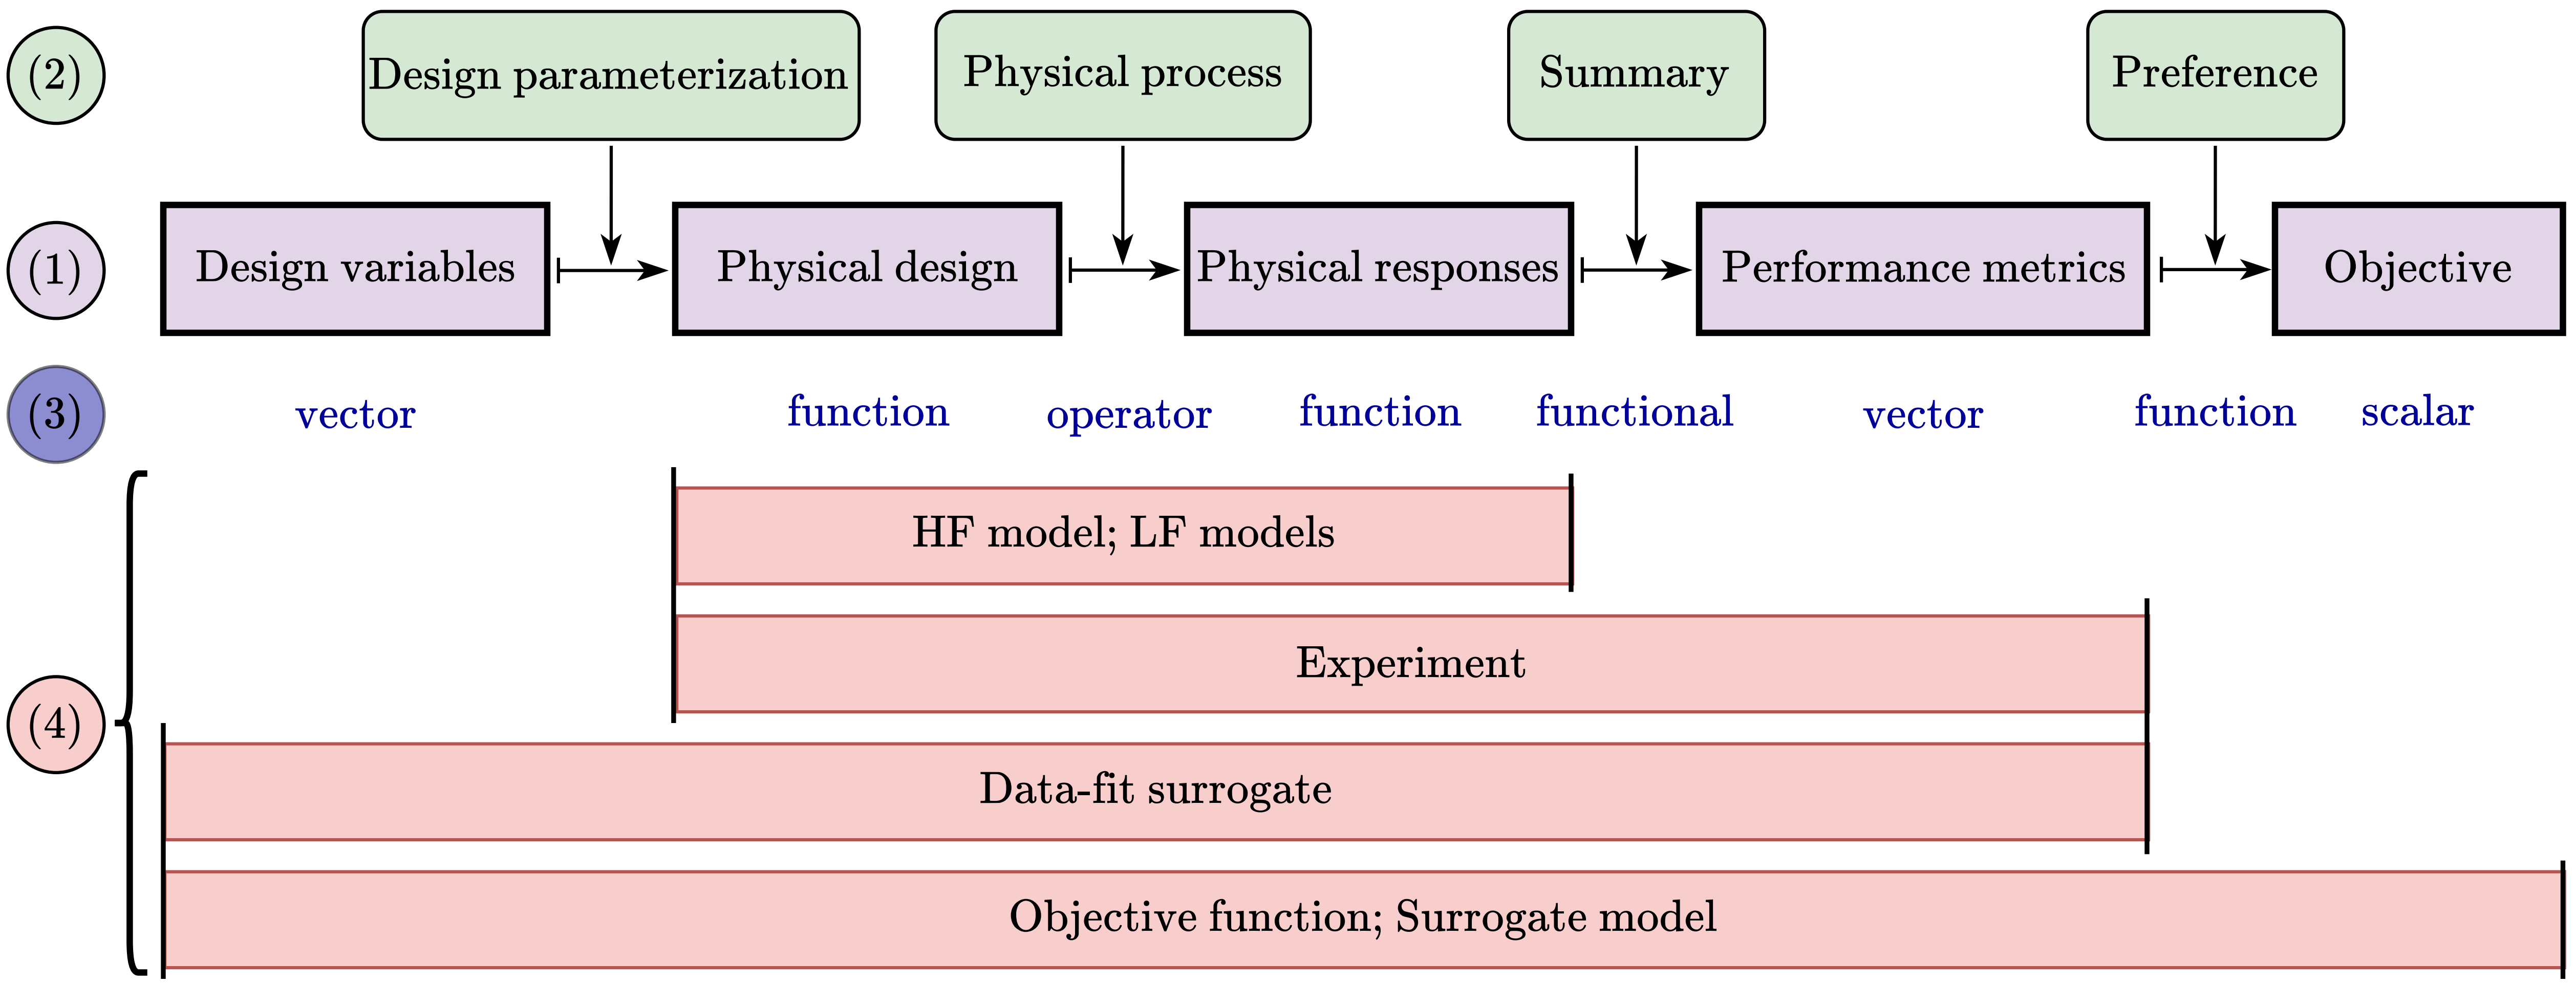
\includegraphics[scale=0.80]{Fig0.png}
	\caption{ Distinction between (a) Surrogate-based optimization, (b) MF optimization, and (c) MF BO optimization.}
	\label{Fig0}
\end{figure*}

% Section 2
\section{Overview of surrogate-based optimization and multi-fidelity Bayesian optimization}\label{Sec2}

\subsection{Surrogate-based optimization and multi-fidelity optimization}\label{Sec21}

The development of surrogate-based optimization in engineering design has received a substantial boost from the work on Design and Analysis of Computer Experiments (DACE) by~\cite{Sacks1989}.
In DACE, a cost-effective Kriging model was used to estimate the output of a computationally intensive computer code.
The best linear unbiased predictor of the Kriging model was obtained by minimizing the mean squared error (MSE) of the predictor.
DACE also introduced some design criteria, such as the integrated MSE, maximum MSE, and expected posterior entropy, to the construction of a computer design capable of making good predictions at unseen input variable vectors.

The use of global function approximations, such as response surfaces and neural networks, to facilitate the optimization process dates back to the 1980s~\citep{Barthelemy1993}.
At that time, there was a limited number of structural optimization applications.
However, the early 1990s~\citep{Sobieski1997} witnessed many applications of the response surface methodology, first introduced by~\cite{Box1951}, to single-discipline and multi-discipline design optimization problems, thanks to the pioneering contributions from research groups at the Virginia Polytechnic Institute and State University, the University of Notre Dame, Rensselaer Polytechnic Institute, Old Dominion University, and the NASA's Langley Research Center~\citep{Viana2014}.
The community also soon recognized a significant limitation of response surface methods -- their applicability to small-scale problems due to the curse of dimensionality~\citep{Barthelemy1993}.
Consequently, attention began to shift away from response surfaces towards alternative approximation methods such as radial basis functions~\citep{Hussain2002}, support vector regression~\citep{Girosi1998}, Kriging~\citep{Cressie1990,Kleijnen2009}, and ensembles~\citep{Goel2007}. 

The applications of Kriging modeling to engineering design optimization gained significant momentum between the late 1990s to the early 2000s~\citep{Torczon1998,Simpson2001}.
In early applications, the best linear unbiased predictor of Kriging served as the objective function.
Minimizing this predictor led to a new design candidate.
This, in turn, updated both the predictor and the current-best solution if the newly proposed design candidate proved superior to the best solution found so far.
By optimizing an aerospike nozzle with three design variables, \cite{Simpson2001} showed that the use of Kriging yielded approximate solutions that were slightly more accurate than those from the response surface methods.
Other works on Kriging focused on how to correct the prediction variance~\citep{Hertog2006} and how to tune its hyperparameters~\citep{Toal2008}.

There are invaluable surveys in the literature that provide comprehensive insights into surrogate-based optimization methods.
\cite{Queipo2005} discussed the fundamental issues arising in surrogate-based analysis and optimization, including the design of experiments, construction of surrogate models, model selection, and sensitivity analysis.
\cite{Wang2006}, from a practitioner’s perspective, provided an overview of how metamodeling techniques can support engineering design optimization.
\cite{Simpson2008} conducted a detailed review of the development of approximation methods in multi-discipline design optimization from 1980 to 2008.
In addition, \cite{Forrester2009} reviewed some state-of-the-art surrogate models and their use in optimization.
\cite{Viana2014} offered an overview of the progression of metamodeling techniques in multi-discipline design optimization.

The use of MF modeling for optimization, termed MF optimization, was initiated by~\cite{Haftka1991} with the deterministic multiplicative MF emulator (Section~\ref{Sec3}).
The objective was to extend the application range of the HF responses by scaling the associated LF responses.
For optimization, this MF emulator imposed first-order consistency conditions, requiring that the HF response and its derivatives at a given design point align with those of the scaled LF response~\citep{Alexandrov2001}.
Sometimes, only the consistency in the HF and scaled LF responses was required~\citep{Rodriguez2001}.
During its early days, MF optimization predominantly focused on a gradient-based optimization approach (Section~\ref{Sec4}), often supplemented by the trust-region framework and deterministic MF emulators~\citep{Alexandrov1998,Alexandrov2000,Alexandrov2001}.
Applications of MF gradient-based optimization were found in supersonic transport design~\citep{Knill1999}, aerodynamic wing design~\citep{Alexandrov2001}, and airfoil design~\citep{Gano2005}.
The development of MF-based optimization methods using deterministic MF emulators can be found in two recent surveys by~\cite{Viana2014} and \cite{Peherstorfer2018}.
%============================================================

%Figure 1
\begin{figure*}
	\centering
	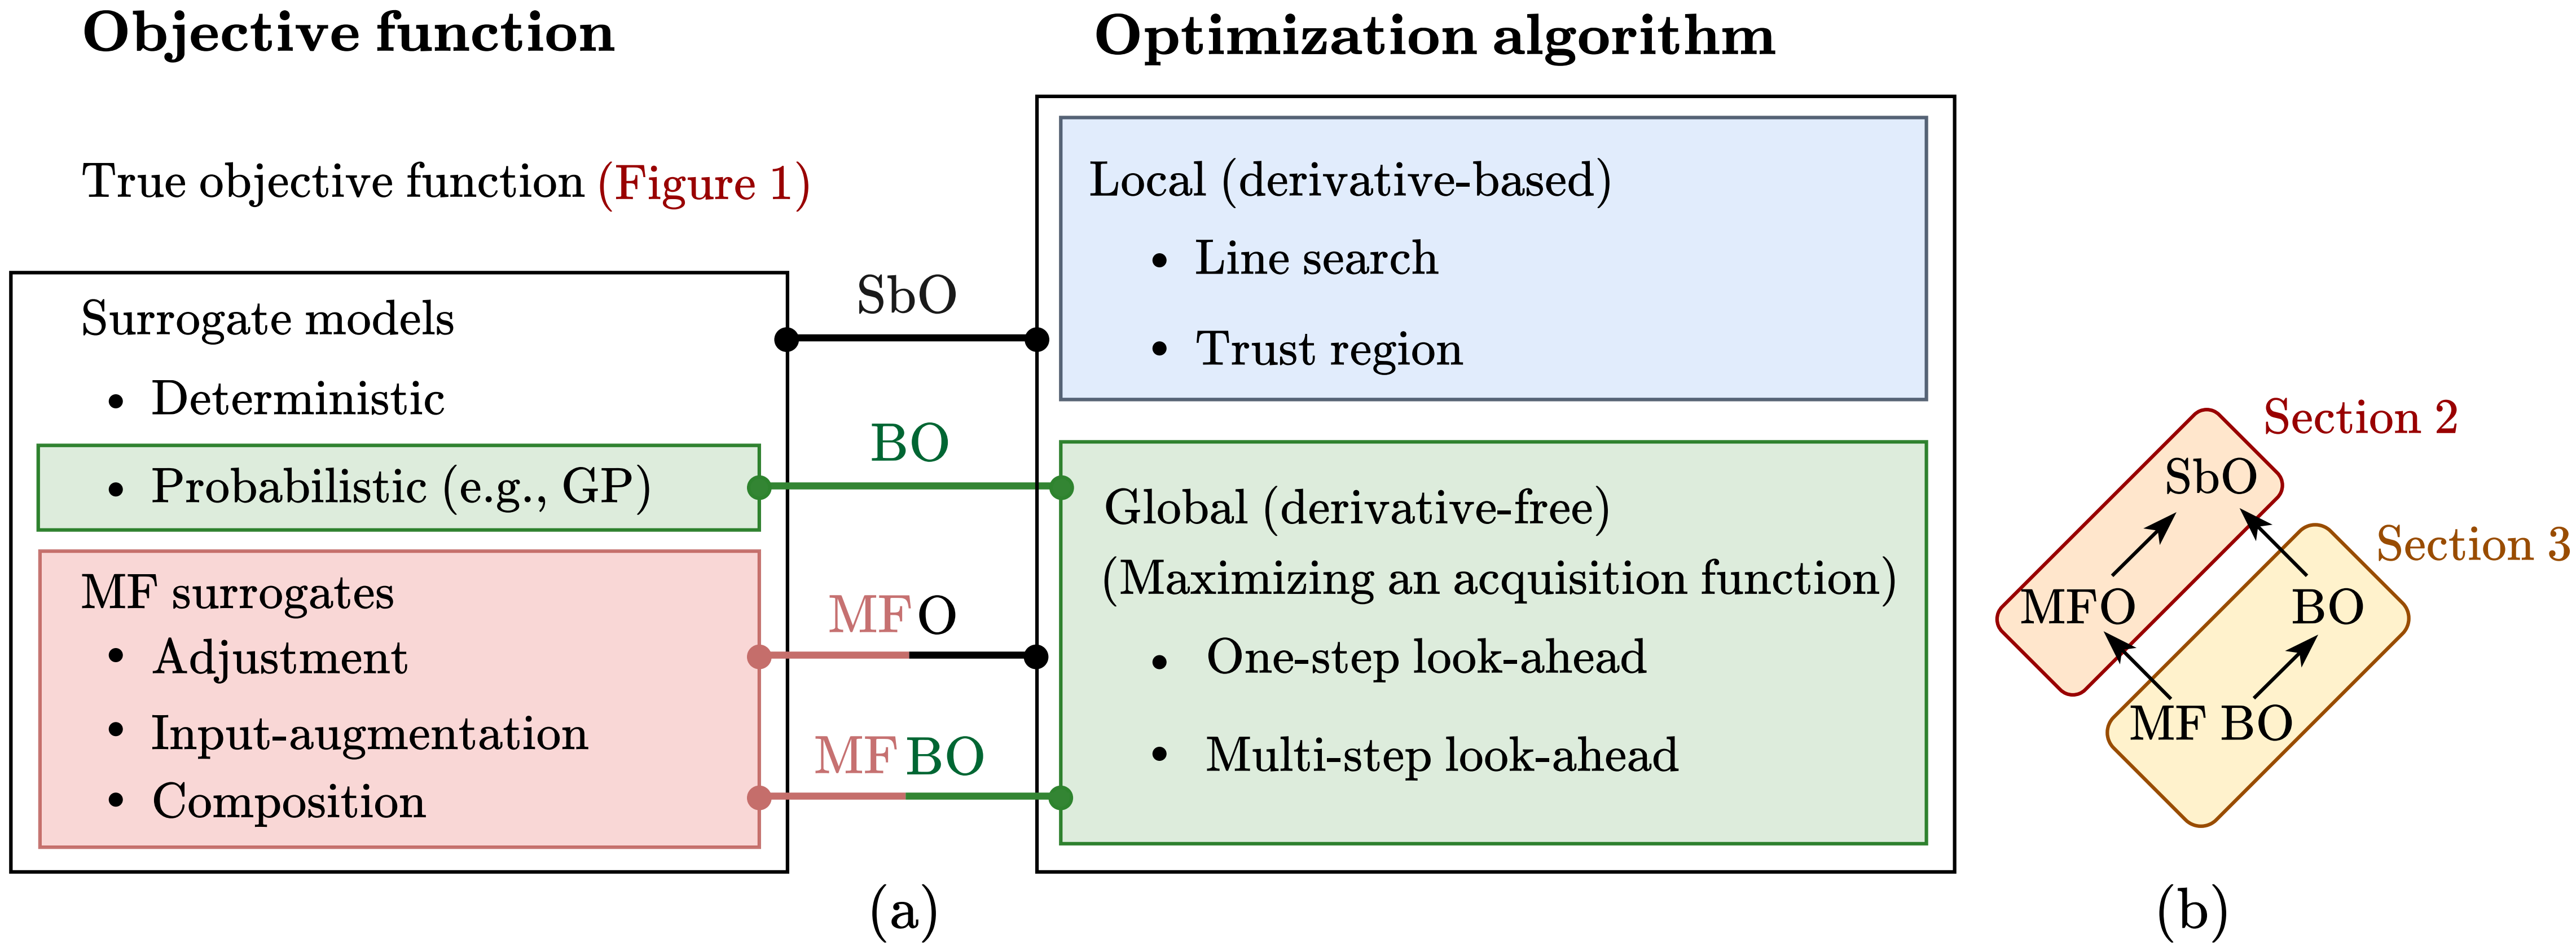
\includegraphics[scale=0.81]{Fig1.png}
	\caption{ Illustration of two consecutive iterates of BO for minimizing a univariate objective function $f(x)$.}
	\label{Fig1}
\end{figure*}

\subsection{Bayesian optimization and multi-fidelity Bayesian optimization}\label{Sec22}

BO was originated by~\cite{Mockus1975} and popularized by~\cite{Jones1998} and their work on the Efficient Global Optimization (EGO) algorithm for problems with expensive-to-compute objective functions.
EGO operates through a sequence of three key steps at each iterate.

In the first step, EGO uses simple Kriging as a stochastic process model for the objective function. The hyperparameters governing this model are determined by maximizing the likelihood of the available training data~\citep{Jones1998}.
This enables the derivation of the best linear unbiased predictor and the associated MSE of the predictor.
Traditionally, in spatial statistics, the best linear unbiased predictor of Kriging is found by minimizing the MSE of the predictor~\citep{Sacks1989,Kleijnen2009}. 
However, within the context of EGO, maximizing the likelihood and minimizing the MSE are equivalent because EGO models the error terms as independent and identically distributed normal random variables~\citep{Jones1998}.

In the second step, EGO formulates what is known as the expected improvement based on (i) the best design point found so far in the training data, (ii) the best linear unbiased predictor, and (ii) the mean squared error of the predictor.
The concept of expected improvement (Section~\ref{Sec611}) strikes a delicate balance between exploiting the information provided by the predictor and exploring uncertain regions within it.

In the third step, EGO maximizes the expected improvement for a new design point and moves to the next iterate.
This new design point is added to the training data, leading to an update of both the Kriging model and the best-found solution.
Notably, maximizing the expected improvement is a more straightforward and computationally efficient process compared to computing derivatives of the costly objective function.
This computational advantage contributes to the overall efficiency of the EGO algorithm.   

While the fundamental concept behind BO closely resembles that of EGO, it is worth noting that BO is the more commonly used term within the fields of statistics and computer science~\citep{Srinivas2010,Bull2011,Snoek2012,Shahriari2016,Frazier2018}.
In BO, a GP model, which is trained by maximizing the likelihood, often serves as the surrogate for the expensive-to-compute objective function, and an acquisition function guides the optimization process.
However, EGO can be considered a specific instance of BO that adopts the expected improvement as the acquisition function.
The interchangeability between Kriging and GP models in the realm of spatial statistics further reinforces the connection between EGO and the broader family of BO algorithms~\citep{Wang2023}.

Figure~\ref{Fig1} shows two consecutive iterates of BO.
In Fig.~\ref{Fig1}(a), BO fits the GP
model for a costly, univariate objective function $f(x)$ to a training data of
four samples (top panel).
It then formulates and maximizes the acquisition function $\alpha(x)$ for a new design point (bottom panel).
In Fig.~\ref{Fig1}(b), BO updates the GP model and reformulates $\alpha(x)$ with the new design point found in the previous iterate.

Mathematically, Algorithm~\ref{Algo1} shows a pseudo-code for solving problem~(\ref{Eq1}) using the generic BO.
The parameters $K$ and $N$ in Step 1 denote the allowable value for the number of BO iterates and the number of initial training samples, respectively.
$\mathcal{D}^{0}$ in Steps 3 and 6 is the initial training data.
$\hat{f}_\text{H}^k({\bf x})$ in Step 10 and $\mathcal{D}^{k}$ in Step 14 are the GP posterior and training data associated with the $k$-th BO iterate.

\begin{algorithm}
	\caption{Pseudo-code for generic BO.}\label{Algo1}
	\begin{algorithmic}[1]
		\State \textbf{Input:} $\mathcal{X}$, $K$, $N$;
		\State Generate $N$ samples of ${\bf x}^i$;
		\State $\mathcal{D}^0 \gets \emptyset$;
		
		\For {$i=1:N$} 
		\State $f^i \gets f_\text{H}({\bf x}^i)$; \textcolor{black}{\Comment{Costly step}}
		\State $\mathcal{D}^0 \gets \mathcal{D}^0 \cup ({\bf x}^i,f^i)$;
		\EndFor
		\State $({\bf x}_{\min},f_{\min}) \gets \min\{f^i,\, i=1,\dots, N\}$;
		
		\For {$k=1:K$} 
		\State Construct $\hat{f}_\text{H}^k({\bf x})$ based on $\mathcal{D}^{k-1}$;
		\State Formulate $\alpha({\bf x})$;
		\State ${\bf x}^{k} \gets \underset{{\bf x}}{\mathrm{argmax}} \ \ \alpha({\bf x})$ s.t. ${\bf x} \in \mathcal{X}$;
		\State $f^{N+k} \gets f_\text{H}({\bf x}^{k})$;
		\textcolor{black}{\Comment{Costly step}}
		\State $\mathcal{D}^k\gets\mathcal{D}^{k-1} \cup ({\bf x}^{k},f^{N+k})$;
		\State $({\bf x}_{\min},f_{\min}) \gets \min\{f^i,\, i=1,\dots, N+k\}$;
		\EndFor
		
		\State \Return $({\bf x}_{\min},f_{\min})$.
	\end{algorithmic}
\end{algorithm}

Over the past decade, BO has experienced remarkable growth in its applications across diverse scientific and engineering disciplines.
BO's unique ability to optimize expensive-to-compute objective functions without relying on their derivative information has made it an invaluable tool of various domains, including machine learning~\citep{Bergstra2011,Klein2017}, aircraft design~\citep{Priem2020,Jim2021}, material design~\citep{Frazier2015,Tran2019,YiZhang2020,Vangelatos2021,Khatamsaz2021b}, experimental design~\citep{Greenhill2020,Lei2021}, material science~\citep{Ueno2016,QLiang2021,Deshwal2021}, structural engineering~\citep{Mathern2021,Kuhn2022,Do2021,Do2022,Do2023}, transportation~\citep{RShi2021}, chemical engineering~\citep{Park2018,KWang2022}, electronics engineering~\citep{Torun2018}, environmental engineering~\citep{Manheim2019}, and  physics~\citep{Yamashita2018,Roussel2021}.

To address a wide range of optimization problems, sophisticated BO algorithms have also been developed.
The first objective of these algorithms is to examine the performance of acquisition functions from different angles, for example, from improvement-based~\citep{Jones1998,Jones2001,Sobester2005,Frazier2008,ZChen2023} and optimistic~\citep{Srinivas2010,Kaufmann2012} to information-based ~\citep{Viana2009,Hennig2012,Lobato2014,ZWang2017} and likelihood-weighted~\citep{Blanchard2021} acquisition functions, or from one-step look-ahead~\citep{Jones1998,Sobester2005} to multi-step look-ahead acquisition functions~\citep{Lam2016,Lee2020,Paulson2022,Gonzalez2016,Jiang2020}.
The second objective of these algorithms is to extend the application of BO to complex scenarios, including constrained problems~\citep{Schonlau1998,Gramacy2011,Picheny2014,Gramacy2016}, high-dimensional problems~\citep{Eriksson2019,Eriksson2021,Daulton2022a}, problems under uncertainty~\citep{Huang2006a,Picheny2013,Forrester2006,Scott2011,Daulton2021,Daulton2022b}, multi-objective problems~\citep{Knowles2006,QZhang2010,Couckuyt2014,Bradford2018,Daulton2020,Picheny2015}, and combinatorial optimization problems~\citep{GomezBombarelli2018,GarridoMerchan2020}.
For further insights into recent advances in BO, the reader may refer to comprehensive surveys and tutorials by~\cite{Shahriari2016}, \cite{Frazier2018}, and \cite{Wang2023}.

The combinations of BO and MF emulators present powerful MF BO approaches to simulation-based optimization~\citep{Huang2006,Forrester2007,Perdikaris2016,Chen2016}.
BO can use the MF emulators to significantly reduce the total evaluation cost associated with fitting surrogate models to the HF samples, i.e., the computational cost to perform Steps 5 and 13 of Algorithm~\ref{Algo1}.
In addition, the optimization process can benefit from the exploitation-exploration trade-off inherent in BO.
Instead of relying excessively on the derivative information of the MF emulators, it can integrate the principles of BO to guide the optimization process using a balanced search of the design space.

Compared to the generic BO outlined Algorithm~\ref{Algo1}, MF BO introduces two significant modifications.
First, it constructs in Step 10 a GP-based MF emulator, leveraging data from simulations across multiple fidelity levels, rather than relying solely on the GP model for the HF simulation.
A widely-used GP-based MF emulator is the autoregressive model~\citep{Kennedy2000}; see Section~\ref{Sec521}.
Second, MF BO develops in Step 11 an acquisition function capable of simultaneously selecting both a new design point and the fidelity level for the simulation to be invoked in Step 13.
The pioneering example of such an acquisition function is the so-called augmented expected improvement~\citep{Huang2006}; see Section~\ref{Sec62}.

The pioneering works by~\cite{Kennedy2000} and~\cite{Huang2006} have initiated three waves of recent research and development efforts of MF BO:
\begin{itemize}
    \item Enhancing MF emulators~\citep{Forrester2007,Qian2008,Han2012,Gratiet2014,Kandasamy2017,Perdikaris2017,Cutajar2019}.
	
    \item Innovating new MF acquisition functions~\citep{Huang2006,Chen2016,Kandasamy2017,YZhang2018,Ghoreishi2019,Ruan2020,Sacher2021,He2021,Renganathan2021,Fiore2023,Huang2023}.
	
    \item Applying MF BO techniques to various fields of engineering and science~\citep{Perdikaris2017,Meliani2019,Tran2020a,Tran2020b,Hebbal2021a,Khatamsaz2021b,Foumani2023,Winter2023}.
	
\end{itemize}
Moreover, recent advances in BO have the potential to further fuel progress in the research and development of MF BO techniques, particularly in solving intricate engineering optimization problems.

In Sections~\ref{Sec3} and \ref{Sec4}, we provide overviews of various MF modeling techniques and MF optimization strategies, respectively.
The goal is to locate MF BO among the rich literature on MF optimization techniques.
%============================================================

% Table 1 
\begin{table*}
	\caption{Published works on additive, multiplicative, hybrid MF modeling techniques.}
	\label{Table1}
	\centering
	\begin{tabularx}{\textwidth}{lX}
		\hline \noalign{\smallskip}
		Type & Reference\\
		\hline \noalign{\smallskip}
		Additive & \cite{Lewis2000,Gano2006b,Viana2009,Palar2016,Zhang2018,Godino2019,Song2019,Kou2019,Meng2020,Viana2014,Durantin2017,Teichert2019,LYan2019,Kennedy2000,Forrester2007,Leary2003,Xiong2008,Kuya2011,Toal2011,Han2012,Keane2012,Goh2013,Zheng2013,Baar2015,Park2017,YZhang2018,Rokita2018,Xiao2018,Jiang2019,Serani2019,Zhou2020,Shu2021,Kaps2022,Toal2023,Xu2023,Ribeiro2023,Peng2023,Wiangkham2023}     \\
		\noalign{\smallskip}
		Multiplicative & \cite{Haftka1991,Chang1993,Goldfeld2005,Hino2006,Sun2010}     \\
		\noalign{\smallskip}
		Hybrid & \cite{Gano2005,Gano2006a,Han2013,Tyan2015,Nguyen2015,Hu2016,Absi2016,Rumpfkeil2017,Bryson2017,Rumpfkeil2019,Wang2021,Qian2008,Gratiet2013,Gratiet2014,Parussini2017,Hao2020,Ji2021,Cheng2021}    \\
		\hline \noalign{\smallskip}
	\end{tabularx}
\end{table*}

% Table 2
\begin{table*}
	\caption{Published works on deterministic and probabilistic MF modeling techniques.}
	\label{Table2}
	\centering
	\begin{tabularx}{\textwidth}{lX}
		\hline \noalign{\smallskip}
		Type & Reference\\
		\hline \noalign{\smallskip}
		Deterministic & \cite{Zhang2018,Godino2019,Song2019,Kou2019,Durantin2017,Han2013,Tyan2015,Nguyen2015,LYan2019,Rumpfkeil2017,Rumpfkeil2019,Wang2021}  \\
		\noalign{\smallskip}
		Probabilistic &    \cite{Kennedy2000,Forrester2007,Xiong2008,Kuya2011,Toal2011,Han2012,Keane2012,Goh2013,Park2017,Serani2019,Qian2008,Gratiet2013,Gratiet2014,Parussini2017,Xiao2018,Ji2021}\\
		\hline \noalign{\smallskip}
	\end{tabularx}
\end{table*}

% Table 3
\begin{table*}
	\caption{Published works on space mapping methods.}
	\label{Table3}
	\centering
	\begin{tabularx}{\textwidth}{lX}
		\hline \noalign{\smallskip}
		Type & Reference\\
		\hline \noalign{\smallskip}
	 	Input-input mapping & \cite{Bandler1994,Bandler2004,Koziel2006,Robinson2008,Tao2019} \\
		\noalign{\smallskip}
		Output-output mapping &  \cite{Zheng2014,Zhou2017,Perdikaris2017,Jiang2018,Cutajar2019,Hebbal2021b,Li2023}   \\
		\hline \noalign{\smallskip}
	\end{tabularx}
\end{table*}
%============================================================

%Figue 2
\begin{figure*}
	\centering
	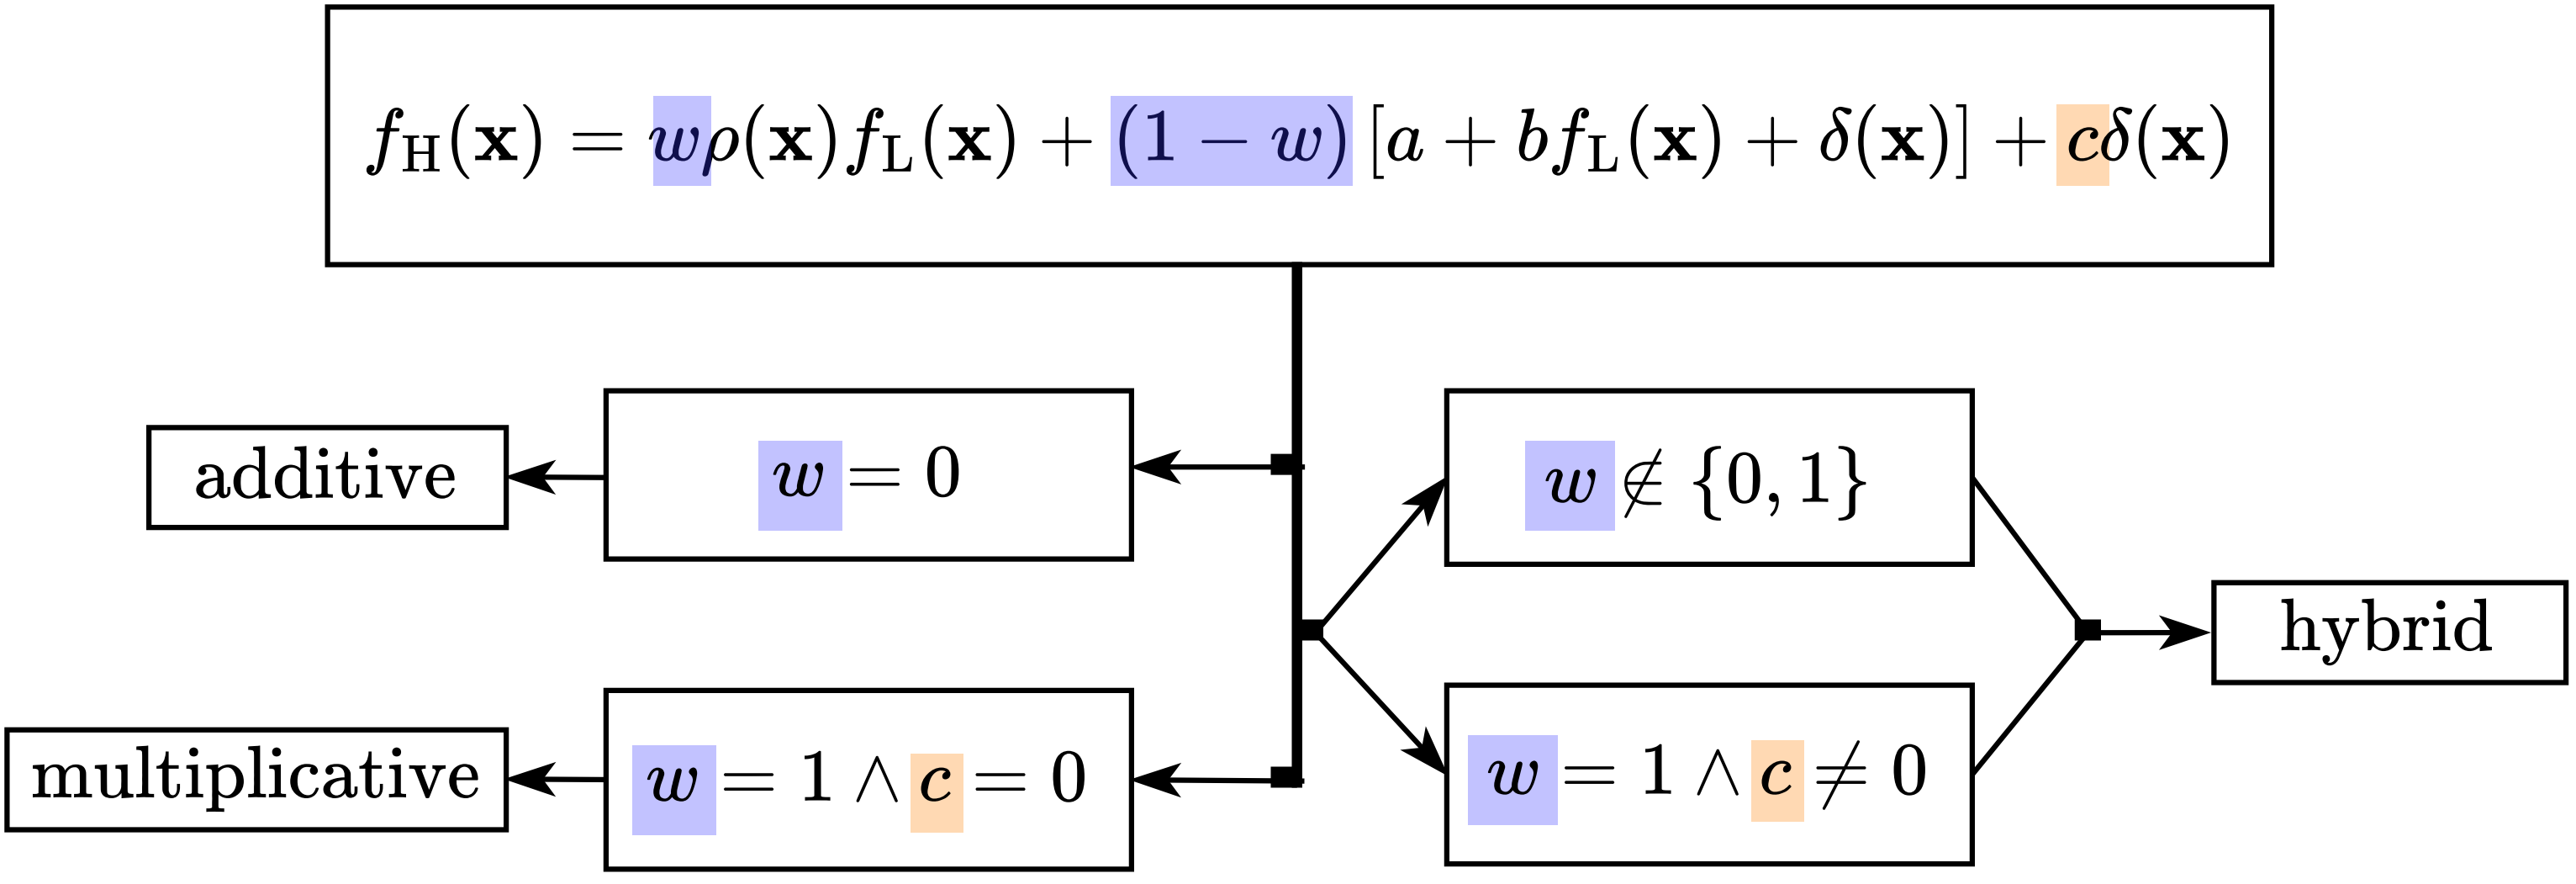
\includegraphics[scale=0.9]{Fig2.png}
	\caption{Additive, multiplicative, and hybrid adjustment methods.}
	\label{Fig2}
\end{figure*}

%Figue 3
\begin{figure*}
	\centering
	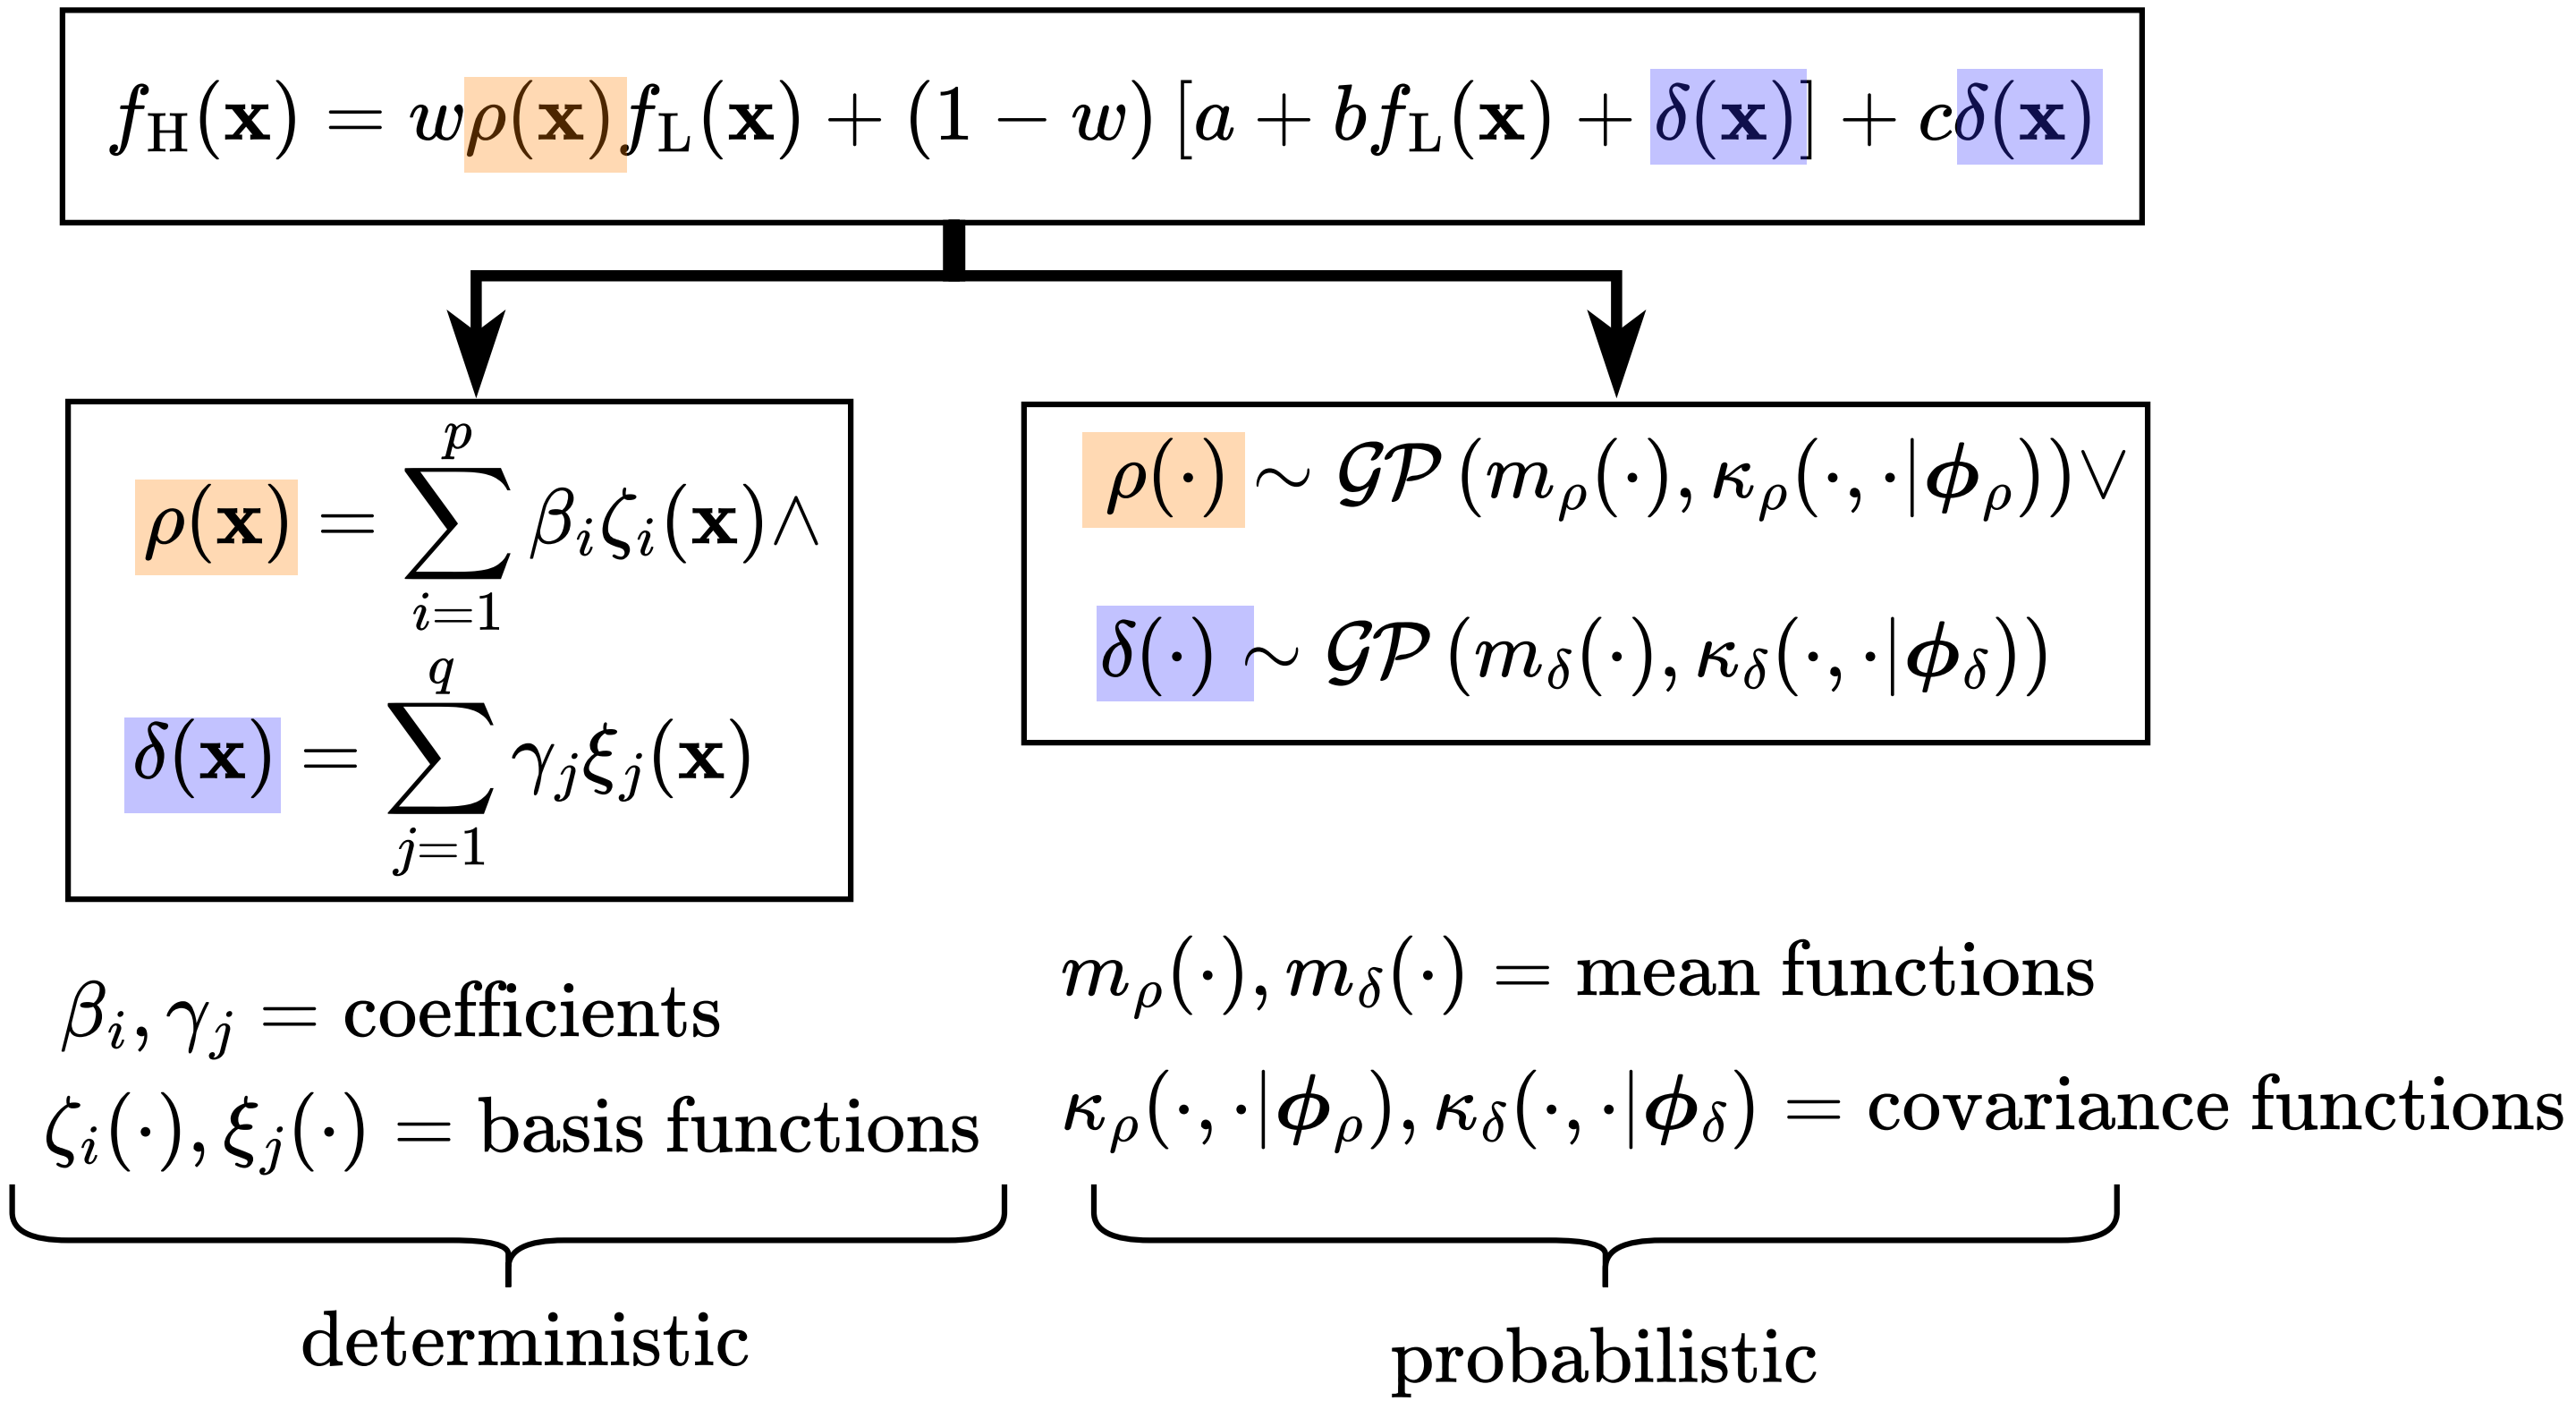
\includegraphics[scale=0.9]{Fig3.png}
	\caption{Deterministic versus probabilistic emulators.}
	\label{Fig3}
\end{figure*}
%============================================================

% Section 3
\section{Overview of multi-fidelity emulators}\label{Sec3}

We can describe most MF emulators for $f_\text{H}({\bf x})$ using the following form:
% Equation 2
\begin{equation}\label{Eq2}
	\begin{aligned}
	f_\text{H}({\bf x})= & \, w \rho({\bf x}) f_\text{L}({\bf x}) + (1-w)\left[a + b f_\text{L}({\bf x}) + \delta({\bf x})\right]\\
	& + c \delta({\bf x}),
\end{aligned}
\end{equation}
where $w$ is a weighting factor, which can be adjusted during the optimization process~\citep{Gano2005}; $\rho({\bf {x}})$ is the correction function~\citep{Haftka1991};  $a$, $b$, and $c$ are three unknown constants; and $\delta({\bf{x}})$ is the discrepancy function~\citep{Kennedy2000}.
By using the form in Eq.~(\ref{Eq2}), we can recover almost all MF emulators listed in a recent review of MF modeling techniques~\citep{Godino2016}.

Based on the values of $w$ and $c$, we can further classify the MF modeling techniques into three types as summarized in Fig.~\ref{Fig2}:
\begin{itemize}
    \item Additive, for $w=0$.

    \item Multiplicative, for $w=1$ and $c=0$.

    \item Hybrid additive/multiplicative, for either $w \notin \{0,1\}$ or $w=1$ and $c \neq 0$.
\end{itemize}
Table~\ref{Table1} enumerates important published works on each type.
Obviously, a substantial portion of these works relies on the additive MF modeling technique.

Based on how $\rho({\bf {x}})$ and $\delta({\bf{x}})$ are modeled, we can also classify the MF modeling techniques into deterministic and probabilistic ones.
The deterministic MF modeling techniques, as described in Fig.~\ref{Fig3}, model both $\rho({\bf {x}})$ and $\delta({\bf{x}})$ as weighted sums of a finite number of basis functions $\zeta_i({\bf {x}})$ and $\xi_j({\bf x})$, respectively.
Commonly used basis functions include monomials~\citep{Zhang2018,Godino2019}, neural networks~\citep{Kou2019}, and radial basis functions~\citep{Tyan2015,Durantin2017}. 
The weight vectors and hyperparameters associated with the basis functions are determined by the least squares or regularized least squares approach. 
In contrast, the probabilistic MF modeling techniques describe $\rho({\bf {x}})$ or $\delta({\bf{x}})$ as a stochastic process, which is often a GP model~\citep{Rasmussen2006}.
The GP-based MF emulator is characterized by a mean function and a kernel function; see Fig.~\ref{Fig3}.   
Table~\ref{Table2} lists important published works on deterministic and probabilistic MF modeling techniques.
Further details on the mathematical foundation of several GP-based MF emulators can be found in~\cite{Brevault2020}.

It is worth noting that the aforementioned classifications do not conflict.
This means an additive (multiplicative, or hybrid) MF emulator can be either deterministic or probabilistic.

Another class of MF modeling techniques known as input-augmentation describes the MF emulators as functions dependent not only on input variables but also on fidelity-level variables.
The fidelity-level variables can be either  categorical~\citep{Foumani2023} or assumed to be continuous for computational efficiency~\citep{Kandasamy2017}.
This differs from the MF emulators in Eq.~(\ref{Eq2}), which are the functions of the input variables only.
Note that most input-augmentation MF emulators are probabilistic.
Section~\ref{Sec56} provides different input-augmentation MF modeling methods.

There also exist MF emulators that are developed from space-mapping methods, specifically the input-input and output-output space mapping MF emulators.
The MF emulators from the input-input space mapping methods often take the form of $f_\text{H}({\bf x}_\text{H})=f_\text{L}({\bf x}_\text{L})$, where ${\bf x}_\text{H}$ is the HF input variable vector, ${\bf x}_\text{L}=g({\bf x}_\text{H})$ is a latent input variable vector obtained via an appropriate function $g(\cdot)$ that maps the input variable space of the HF simulation to that of the LF simulation. 
The MF emulators from the output-output space mapping methods read $f_\text{H}({\bf x}_\text{H})=h\left(f_\text{L}({\bf x}_\text{H})\right)$, where  $h(\cdot)$ is an output-output mapping.
The reader is referred to Table~\ref{Table3} for a list of published works related to space-mapping MF modeling methods.

Since the MF BO algorithms often require GP-based MF emulators, Section~\ref{Sec5} pays special attention to this class of emulators.
%============================================================

% Section 4
\section{Overview of multi-fidelity optimization strategies}\label{Sec4}

The MF optimization strategies take advantage of the relatively low computational cost of the MF emulator and/or its gradient to accelerate the optimization process.
Each MF optimization strategy is characterized by the ways it updates the design points and MF emulators during the optimization process.
There are three different MF optimization strategies, namely gradient-based, model-then-optimize, and sequential model-based optimization approaches.
Notable published works on the algorithms of each approach are listed in Table~\ref{Table4}.

\textbf{Gradient-based approach.} This approach uses a deterministic MF emulator and its derivatives to inform the step length and the search direction. 
This has often been done via the trust-region framework that solves the trust-region subproblem to find a search direction~\citep{Nocedal2006}.
In particular, we first restrict the step size (i.e., define the trust region) for a reliable local model and then find the search direction within the truss region so that it maximizes the reduction of the local model.
In each optimization iteration, the deterministic MF emulator, which can be either additive, multiplicative, or hybrid~\citep{Gano2005}, serves as the local model, while its gradient guides the search for the solution to the trust-region subproblem~\citep{Alexandrov1998,Alexandrov2001,Robinson2008,March2012a}.
Additionally, the MF emulator is used to compute the ratio of actual to predicted improvement for checking whether the new design point is accepted or not, and whether the local model agrees with the actual objective function if the new design point is accepted.
To make the algorithm robust, the MF emulator is occasionally recalibrated using the information from the HF simulation, including the objective function value, gradient, and/or Hessian at a particular design point~\citep{Alexandrov1998,Alexandrov2001}.
To further solve constrained optimization problems, the MF trust-region framework is equipped with a constraint-handling technique, for example, Lagrange multiplier method~\citep{Robinson2008}, augmented Lagrangian method~\citep{Alexandrov2001}, or penalty method with $\text{L}_1$ penalty functions~\citep{Alexandrov2001,Gano2005} or with quadratic penalty functions~\citep{March2012a,Elham2015}.

While the gradient-based MF optimization approach is able to solve high-dimensional optimization problems, its performance is reliant on the adjustment of the trust region and the recalibration of the MF emulator, which require additional costs for calling HF simulations and extracting HF gradients.
The performance also depends on the selection of many tuning parameters underlying the trust-region framework, for example, threshold values for the ratio of actual to predicted improvement, the scaling factors of the trust region size, the tolerance thresholds, and the penalty factors when constrained optimization problems are solved.
	
\textbf{Model-then-optimize approach.} As its name implies, this approach separates the construction of MF emulators from the optimization process.
This approach relies on the condition that the MF emulators must possess sufficient accuracy to ensure both the feasibility and quality of the solution.
However, achieving this level of accuracy may be challenging without the support of an optimization algorithm, primarily because not all regions of the input variable space are useful for optimization.
In practice, focusing on learning a high-confidence region of interest can lead to favorable optimal solutions~\citep{FZhang2023}.
 
The model-then-optimize approach can serve several purposes.
First, it enables an examination of how the initial sampling design impacts solution quality.
Additionally, it becomes particularly useful when the optimization solver is a population-based algorithm~\citep{Viana2009,Leusink2015,Singh2017,Yang2018}.

\textbf{Sequential model-based optimization (SMBO) approach.} This approach iterates between constructing the global surrogate models for costly objective functions and using them to propose new design points via maximizing a acquisition function (i.e., utility function or infill criterion).
In other words, the SMBO approach relies on the acquisition function formulated from the surrogate model to find the search direction and update the surrogate model itself, rather than using the surrogate model and its local information directly.
There are many factors that affect the performance of an SMBO algorithm such as the choice of surrogate models, the selection of acquisition functions, and the construction of initial surrogate models~\citep{Bossek2020}.

The MF BO techniques belong to the SMBO approach that uses a probabilistic MF emulator (often a GP-based MF emulator) as the surrogate model.
This is not only to reduce the computational cost but also to incorporate an automatic exploitation-exploration trade-off into optimization.
Table~\ref{Table4} shows that MF BO techniques have recently attracted a large number of published works on MF optimization.
Most of them, however, focus on solving small- or medium-size problems.
The development of robust MF BO algorithms for large-size optimization problems is still an open research topic~\citep{Frazier2018}. 

In Section~\ref{Sec5}, we describe the first ingredient of MF BO -- GP-based MF emulators.
Its second ingredient -- MF acquisition functions, is the focus of Section~\ref{Sec6}.
% Table 4
\begin{table*}
	\caption{Classification of MF optimization strategies.}
	\label{Table4}
	\centering
	\begin{tabularx}{\textwidth}{lX}
		\hline \noalign{\smallskip}
		Type  & Reference\\
		\hline \noalign{\smallskip}
		Gradient-based  & \cite{Alexandrov1998,Alexandrov2000,Alexandrov2001,Gano2005,Robinson2008,March2011,March2012a,March2012b,Elham2015,Bryson2018,De2020,Wu2022,Zhang2023} \\
		\noalign{\smallskip}
		Model-then-optimize   &  \cite{Viana2009,Leusink2015,Singh2017,Yang2018}   \\
		\noalign{\smallskip}
		\vtop{\hbox{\strut Sequential model-based}\hbox{\strut (MF BO only)}} &  \cite{Sobester2004,Huang2006,Forrester2007,Perdikaris2016,Chen2016,Kandasamy2017,Amrit2018,YZhang2018,Bonfiglio2018a,Bonfiglio2018b,Serani2019,Ghoreishi2019,Bailly2019,Shi2020,Kontogiannis2020,Tran2020a,Tran2020b,Ruan2020,Hao2020,Nachar2020,Fiore2021,Wu2021,He2021,XZhang2021,Shu2021,Khatamsaz2021,Sacher2021,WWu2021,Renganathan2021,Kishi2022,Cheng2022,Foumani2023,Huang2023,Grassi2023,Fiore2023,Shintani2023,Lin2023,Winter2023,Ribeiro2023}   \\
		\noalign{\smallskip}
		\hline 
	\end{tabularx}
\end{table*}
%============================================================

% Section 5
\section{Gaussian process based multi-fidelity emulators}\label{Sec5}

Let ${\bf f}({\bf x})=[f_1({\bf x}),\dots,f_T({\bf x})]^\intercal$, $T \geq 2$, be a vector of $T$ outputs corresponding to $T$ different simulation fidelities for a problem.
We assume that the fidelities share the same inputs, and fidelity levels share the same input variables, and there is no need for an input variable mapping to perform the information transfer between them.
If we sort them in increasing order of fidelity, we have a total of $(T-1)$ LF outputs, and $f_T({\bf x})=f_\text{H}({\bf x})$ is the highest-fidelity output.
Otherwise, there is no obvious hierarchy of these outputs.

Let ${\bf X}_{t}\in \mathbb{R}^{N_t \times d}$, $t=1,\dots,T$ denote the set of $N_t$ input samples for the $t$th fidelity and ${\bf F}_{t}\in \mathbb{R}^{N_t}$ the set of corresponding output observations.
Thus, ${\bf X}=[{\bf X}_1;\dots;{\bf X}_T] \in \mathbb{R}^{\sum_{t=1}^{T} N_t \times d}$ and ${\bf F}=[{\bf F}_1;\dots;{\bf F}_T] \in \mathbb{R}^{\sum_{t=1}^{T} N_t}$ are the sets of input and output data, respectively.
In addition, $\mathcal{D}_t=[{\bf X}_t,{\bf F}_t] \in \mathbb{R}^{N_t \times (d+1)}$ and $D=[\mathcal{D}_1;\dots;\mathcal{D}_T] \in \mathbb{R}^{\sum_{t=1}^{T} N_t \times (d+1)}$ are the training datasets obtained from the $t$th fidelity and from all fidelities, respectively.
%============================================================

\subsection{CoKriging via linear model of coregionalization (LMC)}\label{Sec51}

Without ordering the fidelities, coKriging via linear model of coregionalization (LMC) focuses on the construction of a $T$-variate GP emulator for the output vector ${\bf f}({\bf x})=\left[f_1({\bf x}),\dots,f_T({\bf x})\right]^\intercal$~\citep{Chiles1999,Fricker2013}.
Such a $T$-variate emulator reads
%Equation 3
\begin{equation}\label{Eq3}
	{\bf f}({\bf x}) = {\bf m}({\bf x}) + {\boldsymbol \delta}({\bf x}),
\end{equation}
where ${\bf m}({\bf x})$: $\mathbb{R}^d \mapsto \mathbb{R}^T$ is the mean vector, and ${\boldsymbol \delta}({\bf x})$: $\mathbb{R}^d \mapsto \mathbb{R}^T$ the discrepancy vector.
The construction of a multivariate GP model can be found in Appendix \myNote{refer to Appendix of multivariate GP}.

In LMC, each element of ${\boldsymbol \delta}({\bf x})$ is described by a linear combination of $T$ independent zero-mean GPs with correlation functions $\kappa_1(\cdot,\cdot|{\boldsymbol \phi}_1),\dots,\kappa_T(\cdot,\cdot|{\boldsymbol \phi}_T)$, where ${\boldsymbol \phi}_t$ is the hyperparameter vector of $\kappa_t$.
As a result, ${\boldsymbol \delta}({\bf x}) = {\bf R} {\bf z}({\bf x})$, where ${\bf R} \in \mathbb{R}^{T \times T}$ consists of combination coefficients, and ${\bf z}(\cdot) \sim \mathcal{GP}\left({\bf 0},{\boldsymbol \Sigma}(\cdot,\cdot)\right)$ is a $T$-variate GP with ${\boldsymbol \Sigma}(\cdot,\cdot) = \diag\{\kappa_1(\cdot,\cdot|{\boldsymbol \phi}_1),\dots,\kappa_T(\cdot,\cdot|{\boldsymbol \phi}_T)\}$.
Thus, ${\bf f}(\cdot)$ reads
%Equation 4
\begin{equation}\label{Eq4}
	{\bf f}(\cdot) \sim \mathcal{GP}\left({\bf m}(\cdot),{\bf S}(\cdot,\cdot)\right).
\end{equation}
Here 
${\bf S}(\cdot,\cdot) = {\bf R} {\boldsymbol \Sigma}(\cdot,\cdot) {\bf R}^\intercal = \sum_{t=1}^T {\bf C}_t \kappa_t(\cdot,\cdot|{\boldsymbol \phi}_t)$ is the inter-group covariance matrix, where ${\bf C}_t = {\bf r}_t {\bf r}_t^\intercal$ is the coregionalization matrices and ${\bf r}_t$ the $t$th column of ${\bf R}$.
Thus, an LMC can be considered as a simple factorial coKriging~\citep{Chiles1999}. 
It is also worth noting that ${\bf S}(\cdot,\cdot) \in \mathbb{R}^{T \times T}$ should not be confused with the significantly larger covariance matrix ${\bf K}({\bf X},{\bf X}) \in \mathbb{R}^{\sum_{t=1}^{T}N_t \times \sum_{t=1}^{T}N_t}$, which is used for training and prediction equations.

Once trained, the LMC model can provide the predictions for the outputs of all fidelities at unseen input variable vectors.
See Eqs. of Appendix \myNote{refer to mean and variance equations of multivariate GP}.
%============================================================

\subsection{Auto-regressive model and its variants}\label{Sec52}
\subsubsection{Auto-regressive model (KOH model)}\label{Sec521}

If the fidelities are ordered, the $t$th, $t=2,\dots,T$, fidelity emulator can be described by the $(t-1)$th emulator using the following auto-regressive model~\citep{Kennedy2000}:
% Equation 5 
\begin{subequations}\label{Eq5}
	\begin{align}
		f_t({\bf x}) =
		b_{t-1} f_{t-1}({\bf x}) + \delta_{t}({\bf x}), \ \  t=2,\dots,T \label{Eq5-1},\\
		\text{cov}\left[f_{t}({\bf x}),f_{t-1}({\bf x}')|f_{t-1}({\bf x})\right]=0 
		\label{Eq5-2},
	\end{align}
\end{subequations}
where $b_{t-1}$ is a regression coefficient and $\delta_{t}(\cdot) \sim \mathcal{GP}\left(m_{\delta,t}(\cdot),\kappa_{\delta,t}(\cdot,\cdot|{\boldsymbol \phi}_{\delta,t})\right)$ is the discrepancy function independent of $f_{t-1}(\cdot),\dots,f_{1}(\cdot)$.
Here $b_{t-1}$ and $\delta_{t}(\cdot)$ are similar to $b$ and $\delta(\cdot)$ in Eq.~(\ref{Eq2}), respectively.
$\text{cov}\left[f_{t}({\bf x}),f_{t-1}({\bf x}')|f_{t-1}({\bf x})\right]$ denotes the covariance of two random variables $f_{t}({\bf x})$ and $f_{t-1}({\bf x}')$ given $f_{t-1}({\bf x})$. 
The Markov property in Eq.~(\ref{Eq5-2}) implies that observing $f_{t-1}({\bf x}')$ gives us no information for predicting $f_{t}({\bf x})$ if we observed $f_{t-1}({\bf x})$~\citep{Kennedy2000}.
 
For simplicity, consider two fidelity levels $f_{1}({\bf x})=f_\text{L}({\bf x})$ and $f_{2}({\bf x})=f_\text{H}({\bf x})$.
Eq.~(\ref{Eq5-1}) reads
% Equation 6
\begin{subequations}\label{Eq6}
	\begin{align}
		f_1({\bf x}) & = \delta_1({\bf x}) 
		\label{Eq6-1},\\
		f_2({\bf x}) & = b_{1} f_{1}({\bf x}) + \delta_2({\bf x})
		\label{Eq6-2}.
	\end{align}
\end{subequations}
Let $z_1({\cdot}) \sim \mathcal{GP}\left(0,\kappa_{\delta,1}(\cdot,\cdot|{\boldsymbol \phi}_{\delta,1})\right)$ and $z_2({\cdot}) \sim \mathcal{GP}\left(0,\kappa_{\delta,2}(\cdot,\cdot|{\boldsymbol \phi}_{\delta,2})\right)$, where the kernel functions $\kappa_{\delta,1}$ and $\kappa_{\delta,2}$ are parameterized using the vectors of hyperparameters  ${\boldsymbol \phi}_{\delta,1}$ and ${\boldsymbol \phi}_{\delta,2}$, respectively.
Eq.~(\ref{Eq6}) becomes
% Equation 7
\begin{subequations}\label{Eq7}
	\begin{align}
		f_1({\bf x}) & = m_{\delta,1}({\bf x}) + z_1({\bf x}) 
		\label{Eq7-1},\\
		f_2({\bf x}) & = b_1  m_{\delta,1}({\bf x}) + m_{\delta,2}({\bf x}) + b_1 z_1({\bf x}) + z_2({\bf x})
		\label{Eq7-2}.
	\end{align}
\end{subequations}
This is equivalent to
% Equation 8
\begin{equation}\label{Eq8}
	{\bf f}({\bf x}) =  {\bf m}({\bf x}) + {\bf R} {\bf z}({\bf x}),
\end{equation}
where
% Equation 9
\begin{subequations}\label{Eq9}
	\begin{align}
		{\bf f}({\bf x}) &= \left[f_1({\bf x}),f_2({\bf x})\right]^\intercal 
		\label{Eq9-1},\\
		{\bf m}({\bf x}) &= \left[m_{\delta,1}({\bf x}),b_1  m_{\delta,1}({\bf x}) + m_{\delta,2}({\bf x})\right]^\intercal
		\label{Eq9-2},\\
		{\bf z}({\bf x}) &= \left[z_1({\bf x}),z_2({\bf x})\right]^\intercal, \, {\bf z}(\cdot) \sim \mathcal{GP}\left({\bf 0},{\boldsymbol \Sigma}(\cdot,\cdot)\right)
		\label{Eq9-3},\\
		{\boldsymbol \Sigma}(\cdot,\cdot) &= \left[\begin{matrix}
			\kappa_{\delta,1}(\cdot,\cdot|{\boldsymbol \phi}_{\delta,1}) & 0 \\
			0 & \kappa_{\delta,2}(\cdot,\cdot|{\boldsymbol \phi}_{\delta,2})
		\end{matrix}\right],
		\label{Eq9-4}\\
	 	{\bf R} &= \left[\begin{matrix}
				1 & 0 \\
				b_1 & 1
				\end{matrix}\right]
		\label{Eq-5}.
	\end{align}
\end{subequations}

Thus, ${\bf f}({\bf x})$ in Eq.~(\ref{Eq8}) can be rewritten using the form in Eq.~(\ref{Eq4}) where the inter-group covariance matrix reads
% Equation 10		
\begin{equation}\label{Eq10}
	\begin{aligned}
		{\bf S}(\cdot,\cdot) & = {\bf R} {\boldsymbol \Sigma}(\cdot,\cdot) {\bf R}^\intercal \\
		 & = \left[\begin{matrix}
		 	1 & 0 \\
		 	b_1 & 1
		 \end{matrix}\right] 
		 \left[\begin{matrix}
		 	\kappa_{\delta,1}(\cdot,\cdot|{\boldsymbol \phi}_{\delta,1}) & 0 \\
		 	0 & \kappa_{\delta,2}(\cdot,\cdot|{\boldsymbol \phi}_{\delta,2})
		 \end{matrix}\right]
		 \left[\begin{matrix}
		 	1 & 0 \\
		 	b_1 & 1
		 \end{matrix}\right]^\intercal \\
	 & = \left[\begin{matrix}
	 	\kappa_{\delta,1}(\cdot,\cdot|{\boldsymbol \phi}_{\delta,1}) & b_1 \kappa_{\delta,1}(\cdot,\cdot|{\boldsymbol \phi}_{\delta,1}) \\
	 	b_1 \kappa_{\delta,1}(\cdot,\cdot|{\boldsymbol \phi}_{\delta,1}) & b_1^2 \kappa_{\delta,1}(\cdot,\cdot)+\kappa_{\delta,2}(\cdot,\cdot|{\boldsymbol \phi}_{\delta,2})
	 \end{matrix}\right], 
	\end{aligned}
\end{equation}
which is the inter-group covariance matrix for coKriging derived by~\cite{Forrester2007}.

For the general case of $T$ fidelity levels, the coefficient matrix ${\bf R}$ is a low triangular matrix whose elements are~\citep{Garland2020}
% Equation 11
\begin{equation}
	 r_{ij} = 
	\begin{cases}
		1, & \text{for } i = j, \\
		\prod_{k=j}^{i-1}b_k, & \text{for } i > j, \\
		0, & \text{for } i < j.
	\end{cases}
\end{equation}

The details of training a KOH model for two fidelity levels can be found in~\cite{Forrester2007} or Chapter 8 of the monograph by~\cite{Forrester2008}. 
%============================================================

\subsubsection{Hierarchical Kriging model}\label{Sec522}

\cite{Han2012} proposed the hierarchical Kriging model by making three modifications to the KOH model.
First, they replaced $f_{t-1}({\bf x})$ in Eq.~(\ref{Eq5-1}) with its posterior mean $\mu_{\text{f},t-1}({\bf x})$.
Second, they used $z_{t}({\bf x})$ instead of $\delta_{t}({\bf x})$.
Finally, they modeled the lowest-fidelity emulator $f_1({\bf x})$ as a sum of a constant and a random variable.
Accordingly, the hierarchical Kriging model reads
% Equation 12
\begin{subequations}\label{Eq12}
	\begin{align}
		f_1({\bf x}) & = a + z_1({\bf x}) 
		\label{Eq12-1},\\
		f_t({\bf x}) & =
		b_{t-1} \mu_{\text{f},t-1}({\bf x}) + z_{t}({\bf x}), \ \  t=2,\dots,T
		\label{Eq12-2},
	\end{align}
\end{subequations}
where the constant $a$ is given in Eq.~(\ref{Eq2}).
For the hierarchical Kriging model, we have ${\bf R}={\bf I}$, where ${\bf I}$ is the identity matrix.
%============================================================

\subsubsection{Recursive coKriging model}\label{Sec523}

\cite{Gratiet2014} made two modifications to the KOH model in Eq.~(\ref{Eq5}).
First, they adopted the hybrid additive/multiplicative approach by replacing the regression coefficient $b_{t-1}$, $t=2,\dots,T$, with a correction function $\rho_{t-1}({\bf x})$, which is similar to $\rho_({\bf x})$ in Eq.~(\ref{Eq2}).
Second, they used the GP posterior $\hat{f}_{t-1}({\bf x})$ constructed from the data $\mathcal{D}_{t-1}$ of the $(t-1)$ fidelity instead of $f_{t-1}({\bf x})$.
Accordingly, the recursive coKriging model reads
% Equation 13
\begin{subequations}\label{Eq13}
	\begin{align}
		f_t({\bf x}) =
		\rho_{t-1}({\bf x}) \hat{f}_{t-1}({\bf x}) + \delta_{t}({\bf x}), \ \ t=2,\dots,T \label{Eq13-1},\\
		\text{cov}\left[f_{t}({\bf x}),\hat{f}_{t-1}({\bf x}')|\hat{f}_{t-1}({\bf x})\right]=0 
		\label{Eq13-2}.
	\end{align}
\end{subequations}
Here $\rho_{t-1}({\bf x}) = {\boldsymbol \zeta}_{t-1}^\intercal({\bf x}) {\boldsymbol \beta}_{t-1}$ (see Fig.~\ref{Fig3}) is a linear combination of specified basis functions, and
% Equation 14  
\begin{subequations}\label{Eq14}
	\begin{align}
		\delta_{t}(\cdot) & \sim \mathcal{GP}\left(m_{\delta,t}(\cdot),\kappa_{\delta,t}(\cdot,\cdot|{\boldsymbol \phi}_{\delta,t})\right)
		\label{Eq14-1},\\
		\hat{f}_{t-1}(\cdot) & \sim \mathcal{N}\left(\mu_{\text{f},t-1}(\cdot),\sigma^2_{\text{f},t-1}(\cdot)\right) 
		\label{Eq14-2}.
	\end{align}
\end{subequations}
where $\mu_{\text{f},t-1}(\cdot)$ and $\sigma^2_{\text{f},t-1}(\cdot)$ are the mean function and variance function of the GP posterior $\hat{f}_{t-1}(\cdot)$, respectively.

By using the recursive model, the computational cost for predictions of mean and variance of the highest-fidelity emulator $f_T({\bf x})$ is much less than that of the KOH model while the predictive efficiency is preserved~\citep{Gratiet2014}.
In fact, the KOH model requires the inversion of the $\sum_{t=1}^{T}N_t$-by-$\sum_{t=1}^{T}N_t$ covariance matrix ${\bf K}({\bf X},{\bf X})$ while the recursive model only requires the inversion of $T$ covariance matrices ${\bf K}({\bf X}_t,{\bf X}_t)$ of size $N_t$-by-$N_t$, $t=1,\dots,T$.
%============================================================

\subsubsection{Nonlinear auto-regressive model}\label{Sec524}

Based on the KOH model, \cite{Perdikaris2017} proposed the nonlinear auto-regressive model using the output-output mapping approach; see Section~\ref{Sec3}.
Let $h_{t}(\cdot):\mathbb{R}^{d+1} \mapsto \mathbb{R}$ be the mapping that relates the vector of input and output of the $(t-1)$th fidelity to the output of the $t$th fidelity.
Let ${\bf z}_{t-1}({\bf x})=\left[{\bf x},\hat{f}_{t-1}({\bf x})\right]^\intercal$, where $\hat{f}_{t-1}({\bf x})$ is GP posterior of the $(t-1)$ fidelity emulator.
The nonlinear auto-regressive model reads~\citep{Perdikaris2017}
% Equation 15 
\begin{subequations}\label{Eq15}
	\begin{align}
		f_{t}({\bf x})=h_{t}\left({{\bf z}_{t-1}({\bf x})}\right), \ \  t=2,\dots,T \label{Eq15-1},\\
		\text{cov}\left[f_{t}({\bf x}),{\bf z}_{t-1}({\bf x}')|{\bf z}_{t-1}({\bf x})\right]=0 
		\label{Eq15-2},
	\end{align}
\end{subequations}
where the condition in Eq.~(\ref{Eq15-2}) is equivalent to the Markov property in Eq.~(\ref{Eq5-2}).

In a probabilistic framework, the mapping $h_{t}(\cdot)$ is further modeled as a GP with zero mean and covariance function $\kappa_{\text{h},t}(\cdot,\cdot)$, such that
% Equation 16 
\begin{equation}\label{Eq16}
	h_{t}(\cdot) \sim \mathcal{GP}\left({\bf 0}, \kappa_{\text{h},t}(\cdot,\cdot)\right).
\end{equation} 
Here the kernel function $\kappa_{\text{h},t}(\cdot,\cdot)$ treats the input and output variables separately as
% Equation 17 
\begin{equation}\label{Eq17}
	\begin{aligned}
		\kappa_{\text{h},t}(\cdot,\cdot) & =\kappa_{\text{x},t}(\cdot,\cdot|{\boldsymbol \phi}_{\text{x},t})\kappa_{\text{f},t}(\hat{f}_{t-1}(\cdot),\hat{f}_{t-1}(\cdot)|{\boldsymbol \phi}_{\text{f},t})\\
		& + \kappa_{\delta,t}(\cdot,\cdot|{\boldsymbol \delta}_{\delta,t}),
	\end{aligned}
\end{equation}
where $\kappa_{\text{x},t}$, $\kappa_{\text{f},t}$, $\kappa_{\delta,t}$ are kernel functions corresponding to the input vector ${\bf x}$, the output $f({\bf x})$, and the discrepancy $\delta({\bf x})$ of the $t$th fidelity, respectively.
Since $\hat{f}_{t-1}(\cdot)$ is further defined as a GP prior, $h_{t}(\cdot)$ in Eq.~(\ref{Eq16}) becomes a deep GP model~\citep{Damianou2013}.
 
For $t>2$, we cannot marginalize the likelihood function from Eq.~(\ref{Eq16}) analytically.
As a result, the statistical estimates of $f_{t}({\bf x^\star})$, $t>2$, at an unseen $\bf x^\star$ are obtained via the Monte Carlo integration~\citep{Perdikaris2017}.
%============================================================

\subsection{Bayesian hierarchical model}\label{Sec53}

\cite{Qian2008} performed a full Bayesian treatment for MF modeling using two fidelity levels $f_1({\bf x})$ and $f_2({\bf x})$, where $f_1({\bf x})= f_\text{L}({\bf x})$ and $f_2({\bf x})= f_\text{H}({\bf x})$.
To model the HF emulator $f_\text{2}({\bf x})$, they added a measurement error to the hybrid additive/multiplicative form in Fig.~\ref{Fig2}.
Accordingly, $f_\text{2}({\bf x})$ reads
% Equation 18
\begin{equation}\label{Eq18}
f_\text{2}({\bf x}) = \rho({\bf x})f_\text{1}({\bf x}) + \delta({\bf x})+\varepsilon_2({\bf x}).
\end{equation}
Here the measurement error $\varepsilon_\text{2}(\cdot) \sim \mathcal{N}(0,\sigma^2_{\varepsilon,2})$ is a Gaussian with zero mean and the variance $\sigma^2_{\varepsilon,2} \sim \mathcal{IG}(a_{\varepsilon,2},b_{\varepsilon,2})$, where $\mathcal{IG}(a_{\varepsilon,2},b_{\varepsilon,2})$ denotes the inverse gamma distribution characterized by the shape parameter $a_{\varepsilon,2}$ and the scale parameter $b_{\varepsilon,2}$.

Additionally, the LF emulator is described by
% Equation 19
\begin{equation}\label{Eq19}
	f_1({\bf x}) = {\boldsymbol \zeta}^\intercal({\bf x}) {\boldsymbol \beta}+\varepsilon_1({\bf x}),
\end{equation}
where
% Equation 20
\begin{subequations}\label{Eq20}
	\begin{align}
		{\boldsymbol \zeta}({\bf x})=[1,x_1,\dots,x_d]^\intercal, \ \ {\boldsymbol \beta}=[1,\beta_1,\dots,\beta_d]^\intercal
		\label{Eq20-1},\\
		\varepsilon_1(\cdot) \sim \mathcal{GP}\left(0,\sigma^2_{\varepsilon,1}\kappa_{\varepsilon,1}(\cdot,\cdot|{\boldsymbol \phi}_{\varepsilon,1})\right)
		\label{Eq20-2}.
	\end{align}
\end{subequations}
Here $\sigma^2_{\varepsilon,1}$ is the variance parameter, and $\kappa_{\varepsilon,1}(\cdot,\cdot|{\boldsymbol \phi}_{\varepsilon,1})$ the kernel function conditioned on the hyperparameter vector ${\boldsymbol \phi}_{\varepsilon,1} =[\phi_{\varepsilon,1},\dots,\phi_{\varepsilon,d}]^\intercal$, where $\phi_{\varepsilon,i} \sim \mathcal{G}(a_\varepsilon,b_\varepsilon)$, $i=1,\dots,d$, are gamma distributed parameters.
Furthermore, the coefficient vector ${\boldsymbol \beta}$ in Eq.~(\ref{Eq20-1}) is a Gaussian conditioned on $\sigma^2_{\varepsilon,1}$, such that
% Equation 21
\begin{equation}\label{Eq21}
	{\boldsymbol \beta}|\sigma^2_{\varepsilon,1} \sim \mathcal{N}({\boldsymbol \mu}_\beta,\nu_\beta {\bf I} \sigma^2_{\varepsilon,1}),
\end{equation}
where ${\boldsymbol \mu}_\beta$ and $\nu_\beta$ are the mean vector and a scaling parameter, respectively.

Moreover, the correction function $\rho({\bf x})$ in Eq.~(\ref{Eq18}) is a GP conditioned on the variance value $\sigma^2_\rho$, as
% Equation 22
\begin{equation}\label{Eq22}
	\rho(\cdot) \sim \mathcal{GP}\left(m_\rho|\sigma^2_\rho,\sigma^2_\rho\kappa_\rho(\cdot,\cdot|{\boldsymbol \phi}_\rho)\right).
\end{equation}
Here $m_\rho|\sigma^2_\rho \sim \mathcal{N}(\mu_\rho,\nu_\rho\sigma^2_\rho)$ is the mean parameter, and the kernel function $\kappa_\rho(\cdot,\cdot|{\boldsymbol \phi}_\rho)$ is conditioned on the hyperparameter vector ${\boldsymbol \phi}_\rho =[\phi_{\rho,1},\dots,\phi_{\rho,d}]^\intercal$, where $\phi_{\rho,i} \sim \mathcal{G}(a_\rho,b_\rho)$, $i=1,\dots,d.$ 

Finally, the discrepancy function $\delta({\bf x})$ in Eq.~(\ref{Eq18}) is modeled as
% Equation 23
\begin{equation}\label{Eq23}
	\delta(\cdot) \sim \mathcal{GP}\left(m_\delta|\sigma^2_\delta,\sigma^2_\delta \kappa_\delta(\cdot,\cdot|{\boldsymbol \phi}_\delta)\right).
\end{equation}
Here $m_\delta|\sigma^2_\delta \sim \mathcal{N}(\mu_\delta,\nu_\delta\sigma^2_\delta)$ is the mean parameter, and the kernel function $\kappa_\delta(\cdot,\cdot|{\boldsymbol \phi}_\delta)$ is conditioned on the hyperparameter vector ${\boldsymbol \phi}_\delta =[\phi_{\delta,1},\dots,\phi_{\delta,d}]^\intercal$, where $\phi_{\delta,i} \sim \mathcal{G}(a_\delta,b_\delta)$, $i=1,\dots,d$.

Therefore, the parameters for HF emulator in Eq.~(\ref{Eq18}) consist of the mean parameters ${\boldsymbol \phi}_1 = [{\boldsymbol \beta}^\intercal,m_\rho,m_\delta]^\intercal$, variance parameters ${\boldsymbol \phi}_2 = [\sigma^2_{\varepsilon,2},\sigma^2_{\varepsilon,1},\sigma^2_\rho,\sigma^2_\delta]^\intercal$, and
correlation parameters ${\boldsymbol \phi}_3 = [{\boldsymbol \phi}_{\varepsilon,1}^\intercal,{\boldsymbol \phi}_{\rho}^\intercal,{\boldsymbol \phi}_{\delta}^\intercal]^\intercal$~\citep{Qian2008}. 

It is computationally expensive to predict $f_2$ at an unseen input vector $\bf x^\star$ using a fully Bayesian treatment as it requires the posterior samples of ${\boldsymbol \phi}_1$, ${\boldsymbol \phi}_2$, and ${\boldsymbol \phi}_3$, while sampling the posterior ${\boldsymbol \phi}_3$ is nontrivial.
Thus, \cite{Qian2008} only used the posterior samples of ${\boldsymbol \phi}_1$ and ${\boldsymbol \phi}_2$ for the prediction while fixing ${\boldsymbol \phi}_3$ at its maximum a posteriori probability (MAP) estimate
%============================================================

%Figure 4
\begin{figure}
	\centering
	\includegraphics[scale=0.8]{Fig4.png}
	\caption{General architecture of DGP.}
	\label{Fig4}
\end{figure}

\subsection{Deep multi-fidelity Gaussian process}\label{Sec54}

Deep GP (DGP) describes the mapping between the input variables and the output using the functional of GPs~\citep{Damianou2013}.
Figure~\ref{Fig4} shows the general architecture of DGP of $L$ hidden layers.
In this model, a GP relates two consecutive layers, for example, the GP $f_0$ relates layers 1 and 2.
The architecture in Fig.~\ref{Fig4} is mathematically described as follows:
% Equation 24
\begin{equation}\label{Eq24}
	f({\bf x}) = f_{L-1}\left(\dots f_1(f_0({\bf x}))\right)+\varepsilon_{L-1},
\end{equation}
where $\varepsilon_{L-1}$ is an additive zero-mean Gaussian noise corresponding to layer $L$, and
% Equation 25
\begin{equation}\label{Eq25}
	f_{l-1}(\cdot) \sim \mathcal{GP}\left(0,\kappa_{l-1}(\cdot,\cdot|{\boldsymbol \phi}_{l-1})\right), \ \ l=1,\dots,L,
\end{equation}
where $\kappa_{l-1}(\cdot,\cdot|{\boldsymbol \phi}_{l-1})$ is the kernel function with hyperparameter vector ${\boldsymbol \phi}_{l-1}$.

Using the above DGP modeling framework, \cite{Cutajar2019} proposed the MF DGP in which each layer of DGP corresponds to a fidelity level.
Specifically, layers $2,\dots,L$ shown in Fig.~\ref{Fig4} are associated with fidelities $1,\dots,T-1$, respectively.
This yields the following MF DGP marginal likelihood for the highest-fidelity emulator:
% Equation 26
\begin{equation}\label{Eq26}
	p(f_{T}|{\bf x}) = \int p(f_{T}|f_{T-1})\dots p(f_{1}|{\bf x}) \text{d}f_{1} \dots \text{d}f_{T-1},
\end{equation}
where $p(\cdot)$ denote the probability density function (PDF) of $(\cdot)$.

Since $p(f_{T}|{\bf x})$ is computationally intractable, \cite{Cutajar2019} performed an approximate inference via a so-called doubly stochastic variational inference method~\citep{Salimbeni2017}.

In the MF DGP model, the input vector of a higher fidelity emulator consists of the input variables and the output of the lower fidelity emulator.
Let ${\bf Z}_{t-1} \in \mathbb{R}^{N_t \times {(d+t-1)}}$, $t=1,\dots,T$, denote the set of $N_t$ samples of inducing input variables corresponding to the $t$th fidelity emulator, and ${\bf U}_{t} \in \mathbb{R}^{N_t}$ denote the corresponding function values, where $p({\bf U}_{t}) = \mathcal{N}({\boldsymbol \mu}_{\text{u},t},{\boldsymbol \Sigma}_{\text{u},t})$.
The treatment of inducing input variables is detailed in~\cite{Cutajar2019}.
 
\cite{Cutajar2019} introduced the random vector $\bf u$ such that the joint posterior $p({\bf F}, {\bf U})$ at each fidelity level is associated with a variational lower bound on the marginal likelihood of the exact GP.
Accordingly, the joint posterior at the $t$th fidelity level takes the form of
% Equation 27
\begin{equation}\label{Eq27}
	q({\bf F}_t,{\bf U}_t) = p({\bf F}_t|{\bf U}_t) p({\bf U}_t).
\end{equation}

Marginalizing the inducing input variables from each fidelity level leads to~\citep{Salimbeni2017}
% Equation 28
\begin{equation}\label{Eq28}
	q({\bf F}_t|{\boldsymbol \mu}_{\text{u},t},{\boldsymbol \Sigma}_{\text{u},t}) = \mathcal{N}({\boldsymbol \mu}_{\text{f},t},{\boldsymbol \Sigma}_{\text{f},t}).
\end{equation}

Furthermore, the marginal likelihood is obtained by assuming that the posterior distribution of ${\bf U}_t$, $t=1,\dots,T$, is factorized between the fidelity levels~\citep{Salimbeni2017}, such that
% Equation 29
\begin{equation}\label{Eq29}
	q(f_{T}) = \int \prod_{t=1}^{T} q({\bf F}_t|{\boldsymbol \mu}_{\text{f},t},{\boldsymbol \Sigma}_{\text{f},t}) \text{d}f_{1} \dots \text{d}f_{T-1},
\end{equation}
which is computationally tractable.

Some applications of DGP and MF DGP to engineering design optimization can be found in recent works by~\cite{Hebbal2021a,Hebbal2021b}.
%============================================================

%Figure 5
\begin{figure}
	\centering
	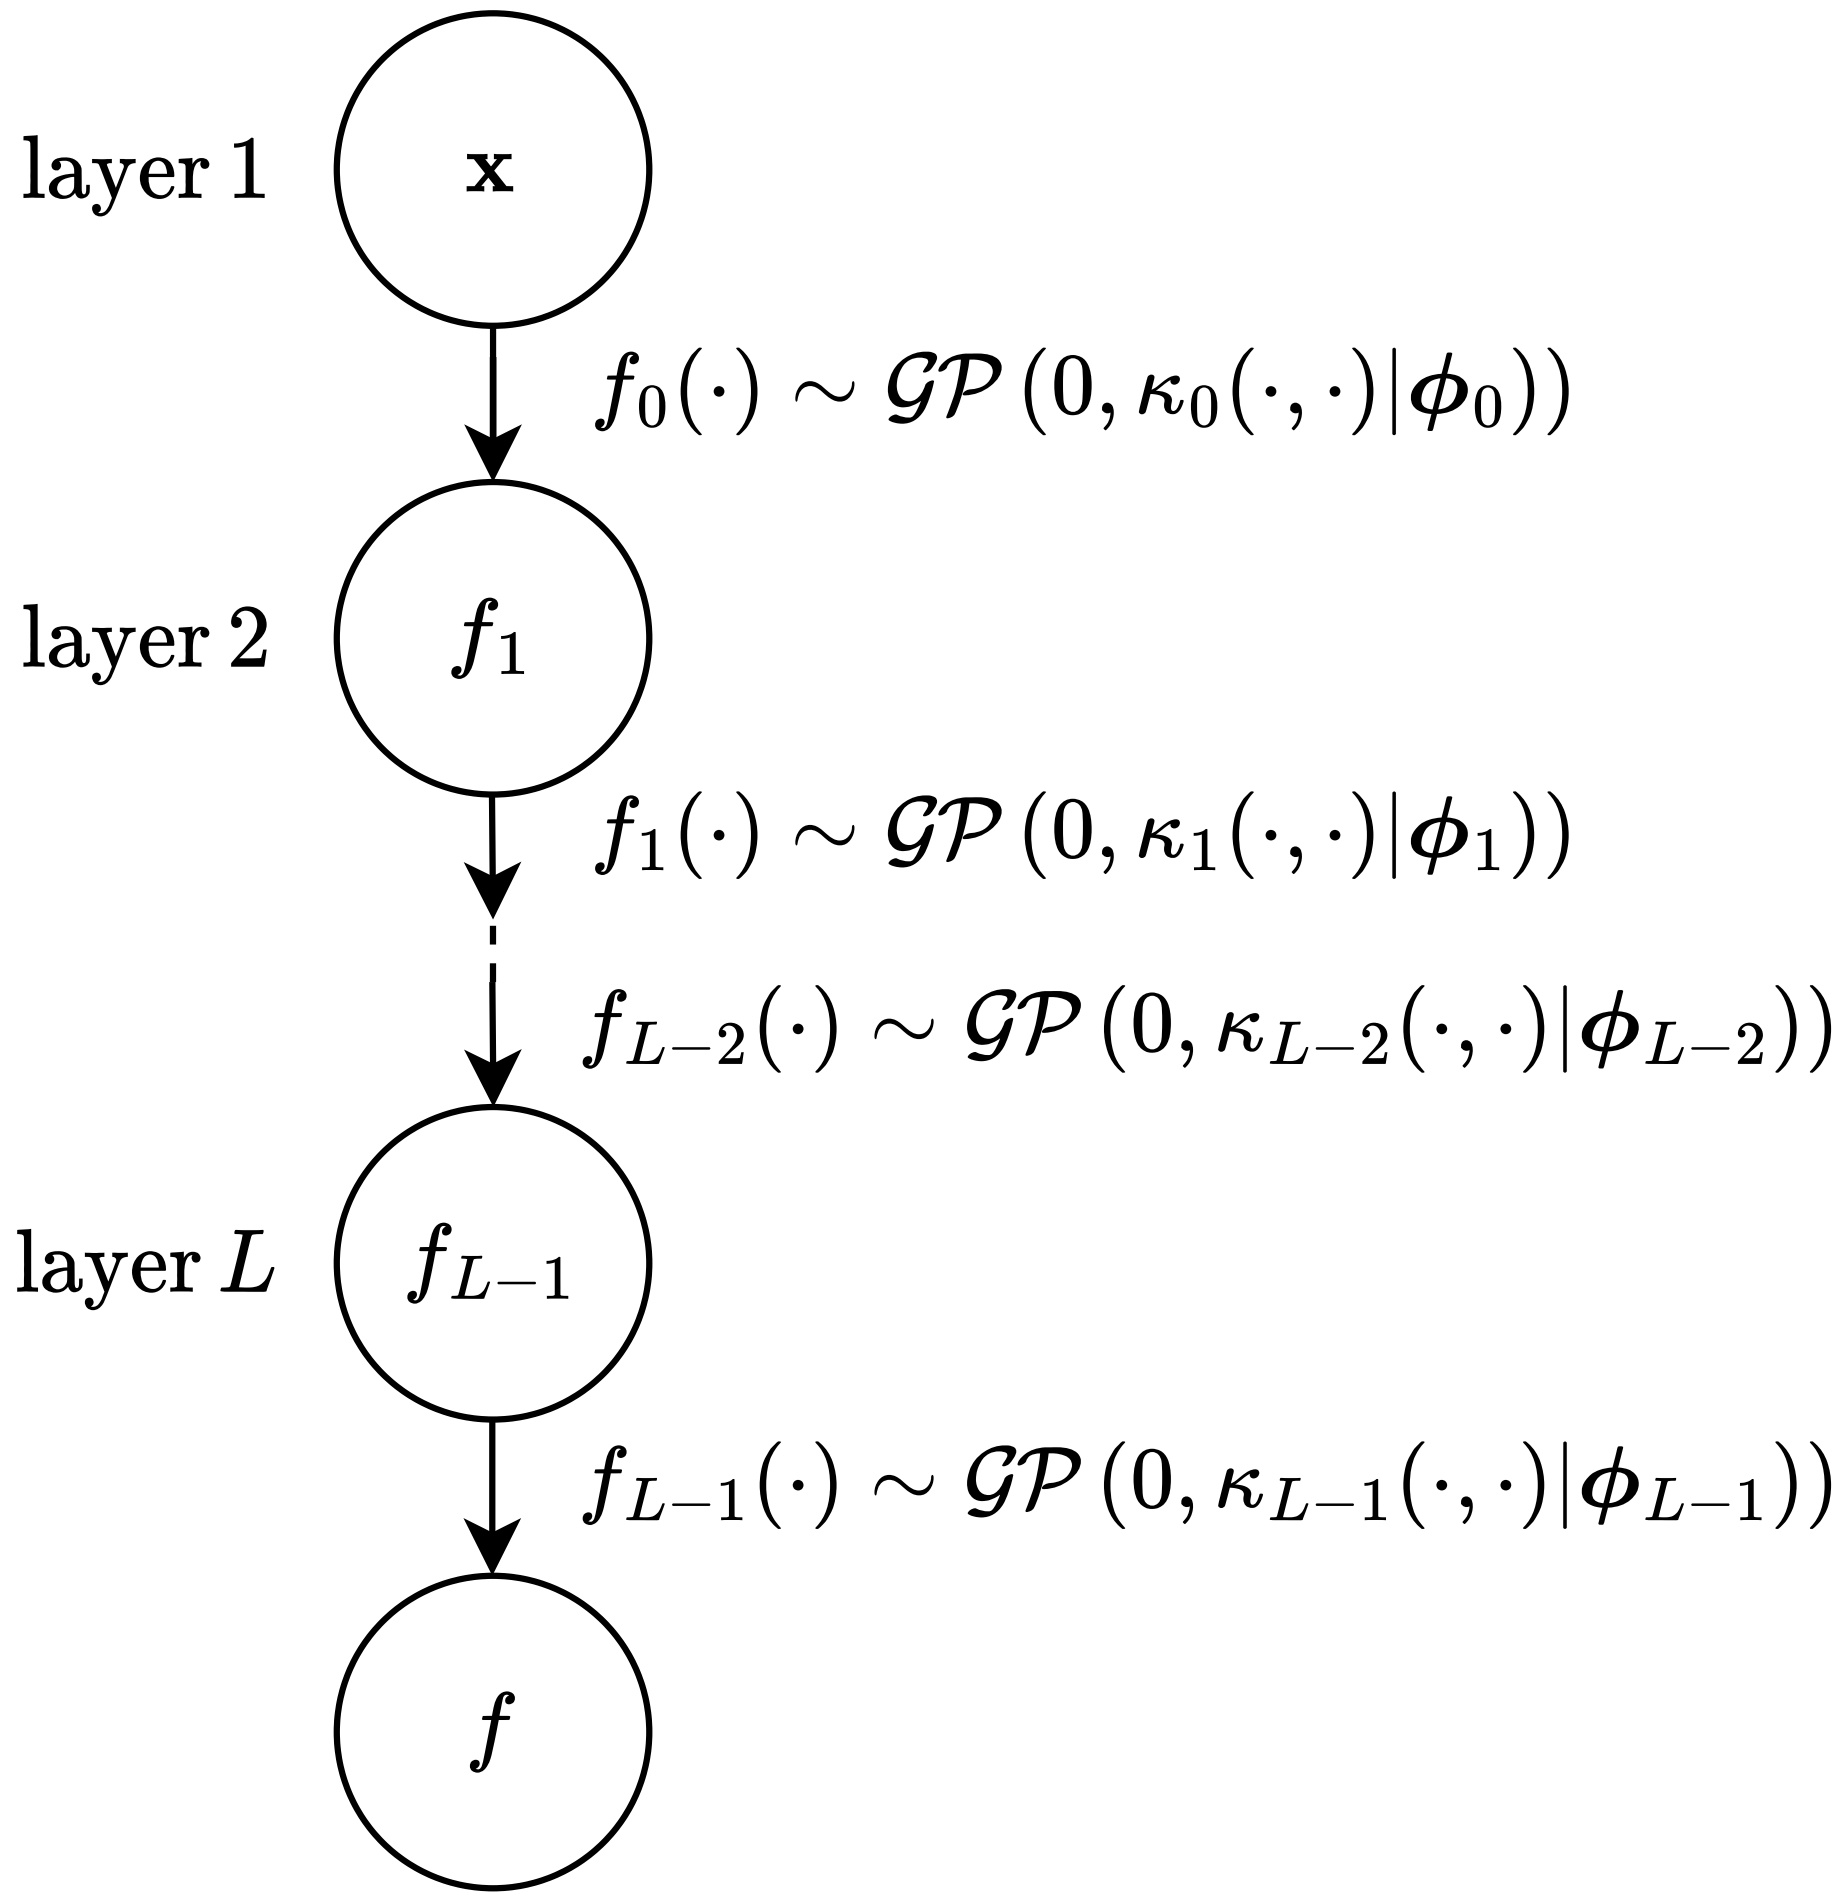
\includegraphics[scale=0.85]{Fig5.png}
	\caption{An example of a directed acyclic for MF modeling.}
	\label{Fig5}
\end{figure}

\subsection{Graphical multi-fidelity Gaussian process (GMGP)}\label{Sec55}

In an attempt to generalize the KOH model, \cite{Ji2021} developed the graphical MF GP (GMGP) valuable in the case that the hierarchy of LF emulators remains unclear.
The GMGP approach involves constructing a directed acyclic graph.
In this graph, each node represents an emulator, and each directed edge connecting two nodes signifies the hierarchy of their fidelities. 
Let $V$ and $T$ denote the set of nodes and the root node for the highest-fidelity emulator.
Let $E$ denote the set of directed edges between nodes.
Consequently, the graph $\mathcal{G}=(V,E)$ serves as the foundation for GMGP.
Figure~\ref{Fig5} shows an example of $\mathcal{G}$.

Consider node $t$ as shown in Fig.~\ref{Fig5}.
Let $\text{Pa}(t)$ denote the sets of its parent nodes.
Let $V_\text{s}$ be the set of all source nodes for the emulators that have lower-fidelity emulator, and $\bar{V}_\text{s} = V \backslash V_\text{s}$ be the set of all non-source nodes.
GMGP models the output from of emulator at node $t$ as the weighted sum of its parent emulators, plus a discrepancy term~\citep{Ji2021}, such that
% Equation 30
\begin{subequations}\label{Eq30}
	\begin{align}
		f_t({\bf x}) = \sum_{t' \in \text{Pa}(t)}
		b_{t'} f_{t'}({\bf x}) + \delta_{t}({\bf x}), \ \  t \in \bar{V}_\text{s}
		\label{Eq30-1},\\
		\text{cov}\left[f_{t}({\bf x}),f_{t'}({\bf x}')|f_{t'}({\bf x})\right]=0, \ \ t' \in  \text{Pa}(t)
		\label{Eq30-2},
	\end{align}
\end{subequations}
where
% Equation 31
\begin{equation}\label{Eq31}
	\delta_{t}(\cdot) \sim \mathcal{GP}\left(m_{\delta,t},\kappa_{\delta,t}(\cdot,\cdot|{\boldsymbol \phi}_{\delta,t})\right), \ \ t \in \bar{V}_\text{s}.
\end{equation}

In addition, a GP prior is assigned to each source node as
% Equation 32
\begin{subequations}\label{Eq32}
	\begin{align}
		f_{t}(\cdot) \sim \mathcal{GP}\left(m_{\text{f},t},\kappa_{\text{f},t}(\cdot,\cdot|{\boldsymbol \phi}_{\text{f},t})\right), \ \ t \in V_\text{s}
		\label{Eq32-1},\\
		\text{cov}\left[f_{t}({\bf x}),f_{t'}({\bf x}')|f_{t'}({\bf x})\right]=0, \ \ t,t' \in  V_\text{s}, \, t \neq t'
		\label{Eq32-2}.
	\end{align}
\end{subequations}

Inspired by~\cite{Gratiet2014}, \cite{Ji2021} also provided the following recursive formulation for the model in Eq.~(\ref{Eq30}):
% Equation 33
\begin{subequations}\label{Eq33}
	\begin{align}
		f_t({\bf x}) = \sum_{t' \in \text{Pa}(t)}
		b_{t'} \hat{f}_{t'}({\bf x}) + \delta_{t}({\bf x}), \ \  t \in \bar{V}_\text{s}
		\label{Eq33-1},\\
		\text{cov}\left[f_{t}({\bf x}),\hat{f}_{t'}({\bf x}')|\hat{f}_{t'}({\bf x})\right]=0, \ \ t' \in  \text{Pa}(t)
		\label{Eq33-2}.
	\end{align}
\end{subequations}
where $\hat{f}_{t'}({\bf x})$ is the GP posterior at node $t'$, which is conditioned on the data for the emulator at $t'$ and those at its ancestor nodes.

The training process of GMGP, and its applications to several numerical experiments and to emulation of heavy-ion collisions are detailed in~\cite{Ji2021}.
%============================================================

\subsection{Input-augmentation multi-fidelity Gaussian process emulators}\label{Sec56}

\subsubsection{Continuous approximation}\label{Sec561}

The GP-based MF emulators described so far have been built in the space of input variables $\bf x$ or the augmented space of input and output variables.
This aligns with the natural tendency to construct GP kernel functions within continuous spaces. \cite{Kandasamy2017}, in contrast, adopted a different approach by constructing GP-based MF emulators as functions of fidelity-level variables and input variables using continuous approximations, leveraging continuous approximations.
This approach, referred to as input-augmentation MF GP modeling, offers a distinct advantage.
It allows for the direct retrieval of the highest-fidelity emulator at any input variable vector by setting the fidelity-level variables to their maximum values.
 
More specifically, \cite{Kandasamy2017} solved the problem of finding the hyperparameter vector ${\bf x}$ for maximizing the validation accuracy $f({\bf x})$.
This validation accuracy depends on ${\bf x}$, the number of data points $t_1$, and the number of optimization iterations $t_2$.
Under the continuous approximations, the validation accuracy can be defined as the slice at ${\bf t}=[t_1,t_2]^\intercal$ of a function $g({\bf t},{\bf x})$ constructed on a larger space, such that
% Equation 34
\begin{equation}\label{Eq34}
	f_{\bf t}({\bf x}) = g({\bf t},{\bf x}).
\end{equation}
Here ${\bf t}=[t_1,t_2]^\intercal$ is the vector of fidelity variables with $t_1 \in [1,N_{\max}]$ and $t_2 \in [1,I_{\max}]$, where $N_{\max}$ and $I_{\max}$ the are allowable numbers of the data points and the optimization iterations.
 
In the probabilistic modeling framework, \cite{Kandasamy2017} assigned a GP prior to  $g({\bf t},{\bf x})$, such that
% Equation 35
\begin{equation}\label{Eq35}
	g(\cdot) \sim \mathcal{GP}\left({\bf 0},\kappa_\text{g}(\cdot,\cdot|{\boldsymbol \phi}_\text{g}\right),
\end{equation}
where the kernel function for continuous ${\bf t}$ takes the form~\citep{Kandasamy2017}
% Equation 36
\begin{equation}\label{Eq36}
	\kappa_\text{g}\left([{\bf t}^\intercal,{\bf x}^\intercal],[{\bf t}'^\intercal,{\bf x}'^\intercal]|{\boldsymbol \phi}_\text{g}\right)=\kappa_\text{t}\left({\bf t},{\bf t}'|{\boldsymbol \phi}_\text{t}\right)\kappa_\text{x}\left({\bf x},{\bf x}'|{\boldsymbol \phi}_\text{x}\right),
\end{equation}
where ${\boldsymbol \phi}_\text{g} = [{\boldsymbol \phi}_\text{t}^\intercal,{\boldsymbol \phi}_\text{x}^\intercal]^\intercal$ denotes the hyperparameter vector of $\kappa_\text{g}$ 

Similar methods for tuning the hyperparameters of machine learning models can be found in~\cite{Poloczek2017} and \cite{JWu2020}.
%============================================================

\subsubsection{Use of discrete kernels}\label{Sec562}

Instead of using the continuous approximations, other works have focused on developing discrete kernels $\kappa_\text{t}\left({\bf t},{\bf t}'|{\boldsymbol \phi}_\text{t}\right)$, where ${\bf t} \in \mathbb{Z}^{n_t}$ and each element $t_i$, $i=1,\dots,n_t$, has a total of $l_i$ discrete levels.

\cite{Zhou2011} proposed the hypersphere decomposition kernel in which the discrete kernel $\kappa_\text{t}\left({\bf t},{\bf t}'|{\boldsymbol \phi}_\text{t}\right)$ is defined as the product between the univariate kernels of its elements.
Furthermore, the univariate kernel of each element is modeled as the Euclidean scalar product between the hypersphere mappings.
Accordingly, the discrete kernel reads
% Equation 37
\begin{subequations}\label{Eq37}
	\begin{align}
		\kappa_\text{t}\left({\bf t},{\bf t}'|{\boldsymbol \phi}_\text{t}\right) & = \prod_{i=1}^{n_t}\kappa(t_i,t_i'|{\boldsymbol \phi}_{\text{t},i})
		\label{Eq37-1},\\
		\kappa(t_i,t_i'|{\boldsymbol \phi}_{\text{t},i})& =\varphi(t_i|{\boldsymbol \phi}_{\text{t},i})^\intercal \varphi(t_i'|{\boldsymbol \phi}_{\text{t},i})
		\label{Eq37-2},
	\end{align}
\end{subequations}
where $\varphi(t_i|{\boldsymbol \phi}_{\text{t},i})$ maps each of  the $l_i$ levels of $t_i$ onto a point lying on the surface of a $l_i$-dimensional hypersphere.
See~\cite{Zhou2011} for the details of this mapping.

\cite{Roustant2020} also provided the parsimonious form of $\kappa(t_i,t_i'|{\boldsymbol \phi}_{t,i})$ in Eq.~(\ref{Eq37-2}) called the compound symmetry kernel.
$\kappa(t_i,t_i'|{\boldsymbol \phi}_{t,i})$ assumes a common correlation for all levels, such that
% Equation 38
\begin{equation}\label{Eq38}
	\kappa(t_i,t_i'|{\boldsymbol \phi}_{\text{t},i}) = 
	\begin{cases}
		\sigma_{\text{t},i}^2, & \text{for } t_i = t_i', \\
		\theta \sigma_{\text{t},i}^2, & \text{for } t_i \neq t_i',
	\end{cases}
\end{equation}
where $\theta \in (-1/(l_i-1),1)$.

Alternatively, \cite{Foumani2023} mapped the vector ${\bf t}$ of fidelity variables onto a latent space of continuous variables ${\bf z}({\bf t})$.
In particular, ${\bf t}$ is related to ${\bf z}$ via a mapping matrix ${\bf A}$, as~\citep{Foumani2023,Oune2021}
% Equation 39
\begin{equation}\label{Eq39}
	{\bf z}({\bf t}) = {\boldsymbol \zeta}({\bf t}) {\bf A},
\end{equation}
where ${\boldsymbol \zeta}({\bf t})$ is the prior vector representation of ${\bf t}$ that is defined using either the random initialization or the one-hot encoding technique, and the elements of ${\bf A}$ are found via maximum likelihood estimation when some data points are observed~\citep{Oune2021}.
Related mapping techniques and their applications in engineering design can be found in~\cite{Deng2017,YZhang2020,GarridoMerchan2020,Pelamatti2021,Vangelatos2021,LWang2021,Saves2023}.

Once the mapping ${\bf z}({\bf t})$ has been established, the discrete kernel function $\kappa_\text{t}\left({\bf t},{\bf t}'|{\boldsymbol \phi}_t\right)$ in Eq.~(\ref{Eq36}) becomes~\citep{Foumani2023}
% Equation 40
\begin{equation}\label{Eq40}
	\kappa_\text{t}\left({\bf t},{\bf t}'|{\boldsymbol \phi}_\text{t}\right)=\kappa_\text{z}\left({\bf z}({\bf t}),{\bf z}({\bf t}')|{\boldsymbol \phi}_\text{z}\right),
\end{equation}
where $\kappa_\text{z}\left({\bf z}({\bf t}),{\bf z}({\bf t}')|{\boldsymbol \phi}_\text{z}\right)$ is the kernel function defined in the continuous space of ${\bf z}$.

To select an appropriate discrete kernel for a specific problem, \cite{Pelamatti2021} compared the main characteristics of the hypersphere decomposition kernel, compound symmetry kernel, and latent mapping kernel.
They also provided the number of hyperparameters for each of these kernels with respect to the number of discrete levels.
%============================================================

% Section 6
\section{Acquisition functions}\label{Sec6}

An acquisition function serves as a metric measuring our expectations regarding the potential improvement in a solution at each point in the input variable space.
In this context, ``solution improvement" is broadly defined, encompassing the improvement in the objective function value, the information gain on the true minimizer, or the information gain on the true minimum.
Maximizing the acquisition function guides BO toward a new design point with the highest score of solution improvement.
In this section, we first review widely-used acquisition functions for generic BO provided in the literature~\citep{Shahriari2016,Frazier2018,Wang2023} (Section~\ref{Sec61}).
We then describe how we can modify these acquisition functions for use of MF BO (Section~\ref{Sec62}), followed by a brief discussion of optimization algorithms to maximize the acquisition functions (Section~\ref{Sec63}).
We finally discuss the portfolio of different design points when maximizing a set of multiple acquisition functions (Section~\ref{Sec64}).
%============================================================

\subsection{Acquisition functions for Bayesian optimization}\label{Sec61}
\subsubsection{One-step look-ahead acquisition functions}\label{Sec611}

The class of one-step look-ahead (or myopic) acquisition functions selects a new design point using a utility measure, without forecasting the potential impact of all future selections beyond the immediate next selection.
The acquisition functions in this class include improvement-based acquisition functions, optimistic acquisition functions, and information-based acquisition functions~\citep{Shahriari2016}.

Assume that we are at the $k$th iterate of BO and wish to select the new design point ${\bf x}^{k}$; see Algorithm~\ref{Algo1}.
What we currently know are the GP posterior $\hat{f}_\text{H}^k({\bf x})$ constructed from the data $\mathcal{D}^{k-1}$ from the previous iterate and, under noise-free observation, the best solution we found so far $({\bf x}_{\min}, f_{\min})$.
Denoted by $\mathcal{D}^{k}$ the data after the $k$th iterate has completed, we have $\mathcal{D}^{k} = \mathcal{D}^{k-1} \cup ({\bf x}^{k},f_\text{H}({\bf x}^{k}))$.

In the following, we describe well-established improvement-based acquisition functions, including the probability of improvement~\citep{Kushner1964}, expected improvement~\citep{Mockus1975,Jones1998}, weighted expected improvement~\citep{Sobester2005}, and knowledge gradient~\citep{Frazier2008}.
We then delve into the realm of optimistic acquisition functions, specifically focusing on the negative lower confidence bound, which is derived from the GP upper confidence bound~\citep{Srinivas2010}.
We finally describe several prominent information-based acquisition functions, including  Thompson sampling~\citep{Agrawal2012}, informational approach to global optimization~\citep{Villemonteix2009}, entropy search~\citep{Hennig2012}, predictive entropy search~\citep{Lobato2014}, and max-value entropy search~\citep{ZWang2017}.

\noindent
\textbf{Improvement-based acquisition functions}.

Improvement-based acquisition functions arises from a thought experiment in which we expect that the new design point to be better than the best objective function value $f_\text{min}$ we observed so far.
Consequently, we can define the following solution improvement measure $I({\bf x})$ for minimization problems:
% Equation 41
\begin{equation}\label{Eq41}
	I({\bf x}) = \max{\left(f_\text{min}-f({\bf x}),0\right)}.
\end{equation}

Probability of improvement (PI)~\citep{Kushner1964}, one of the earliest improvement-based acquisition functions, measures the probability that $I({\bf x})$ is positive.
This is equivalent to the chance of having a solution improvement.
When conditioned on the current GP posterior, PI can be expressed in the following analytical form:
% Equation 42
\begin{equation}\label{Eq42}
	\alpha({\bf x}) = \mathbb{P}\left[I({\bf x})>0|\hat{f}_\text{H}^k({\bf x})\right]=\Phi\left(\frac{f_\text{min}-\mu_\text{f}^k({\bf x})}{\sigma_\text{f}^k({\bf x})}\right),
\end{equation}
where $\Phi(\cdot)$ is the standard normal cumulative distribution function (CDF), and $\mu_\text{f}^k({\bf x})$ and $\sigma_\text{f}^k({\bf x})$ are the mean and standard deviation of $\hat{f}_\text{H}^k({\bf x})$ given in Eq.~, respectively \myNote{refer to mean and variance equations of univariate GP}.

While maximizing PI tends to reduce the solution over time, it does not necessarily result in a substantial improvement in the objective function.
This is due to the fact that PI is not a direct quantitative measure of solution improvement~\citep{Kochenderfer2019}.
A more detailed exploration of how PI impacts solution improvement can be found in in~\cite{Jones2001}.

Expected improvement (EI)~\citep{Mockus1975,Jones1998} is an improvement-based acquisition function that quantifies the solution improvement.
As its name suggests, EI calculates the expected value of the improvement $I({\bf x})$, given the current GP posterior.
Mathematically, EI reads
% Equation 43
\begin{equation}\label{Eq43}
	\begin{aligned}
		\alpha({\bf x}) & = \mathbb{E}\left[I({\bf x})|\hat{f}_\text{H}^k({\bf x})\right]\\
		& =\left( f_\text{min}-\mu_\text{f}^k({\bf x})\right)\Phi\left(\frac{f_\text{min}-\mu_\text{f}^k({\bf x})}{\sigma_\text{f}^k({\bf x})}\right)\\
		&+\sigma_\text{f}^k({\bf x})\phi\left(\frac{f_\text{min}-\mu_\text{f}^k({\bf x})}{\sigma_\text{f}^k({\bf x})}\right),
	\end{aligned}
\end{equation}
where $\phi(\cdot)$ denotes the standard normal PDF of $(\cdot)$.
This analytical form is derived using integration by parts~\citep{Jones1998,Kochenderfer2019}.

EI provides a way to conceptualize the balance between exploitation and exploration in optimization.
In the EI expression, the first term embodies exploitation, guiding the search towards a new design point with a high likelihood of improvement.
Meanwhile, the second term embodies exploration, directing the search to regions where there is considerable uncertainty in the prediction of the objective function.
However, EI does not grant us direct control over the exploitation-exploration balance when necessary
For example, it is preferable to bias exploitation if the objective function tends to be unimodal. Conversely, exploration can work well if the objective function is extremely multimodal~\citep{Sobester2005}.

To gain control over the exploitation-exploration balance, \cite{Sobester2005} introduced the weighted EI (WEI) as a weighted sum of the two terms of EI.
WEI reads
% Equation 44
\begin{equation}\label{Eq44}
	\begin{aligned}
		\alpha({\bf x}) & = w\left( f_\text{min}-\mu_\text{f}^k({\bf x})\right)\Phi\left(\frac{f_\text{min}-\mu_\text{f}^k({\bf x})}{\sigma_\text{f}^k({\bf x})}\right)\\
		&+(1-w)\sigma_\text{f}^k({\bf x})\phi\left(\frac{f_\text{min}-\mu_\text{f}^k({\bf x})}{\sigma_\text{f}^k({\bf x})}\right),
	\end{aligned}
\end{equation}
where the weighting factor $w \in [0,1]$.

While $w$ can theoretically vary over $[0,1]$, it is worth noting that maximizing WEI only results in a new design point for a relatively small range of $w$~\citep{Ath2021}.
By carefully investigating this phenomenon, \cite{Ath2021} recommended restricting the choice of $w$ to the interval $[0.185,0.5]$ that guarantees the selection of a new design point lying on the Pareto front of the solutions found so far.

Knowledge gradient (KG)~\citep{Frazier2008} is another improvement-based acquisition function closely related to EI.
However, KG introduces a departure from one of the key assumptions underlying EI.
Particularly, KG operates independently of the best-known objective function value observed so far.
This is justified by considering that the best solution might possess some level of uncertainty relative to EI.

Let $\mu_\text{f}^{k+1}({\cdot})$ be the posterior mean trained from $\mathcal{D}^{k}$, which is formed by appending the unknown point $({\bf x}^k,f_\text{H}({\bf x}^k))$ to the data $\mathcal{D}^{k-1}$ we have so far.
Let ${\bf x}_{\star}^k$ denote the minimizer of the posterior mean $\mu_\text{f}^k({\cdot})$ trained from $\mathcal{D}^{k-1}$.
The KG acquisition function for finding ${\bf x}^k$ is defined as~\citep{Frazier2008}
% Equation 45
\begin{equation}\label{Eq45}
	\alpha({\bf x}) = \mathbb{E}\left[\mu_\text{f}^k({\bf x}_{\star}^k)-\mu_\text{f}^{k+1}({\bf x})\right].
\end{equation}

Because $\mu_\text{f}^{k+1}({\bf x})$ is analytically intractable, the simplest way to estimate KG for a value ${\bf x}$ is via Monte Carlo simulation.
In fact, $\mu_\text{f}^{k+1}({\bf x})$ is an implicit function of the point $({\bf x},f_\text{H}({\bf x}))$ that integrates over all possible values of $f_\text{H}({\bf x})$ under the GP posterior $\hat{f}_\text{H}^k({\bf x})$~\citep{Frazier2018}.

\noindent
\textbf{Optimistic acquisition functions}.

The use of confidence bounds is a popular way to negotiate exploration and exploitation in multi-armed bandit problems~\citep{Lai1985,Auer2002}.
This is underpinned by the concept of embracing optimism in the face of uncertainty~\citep{Shahriari2016}. 
In the context of GP-based optimization, \cite{Srinivas2010} proposed the GP upper confidence bound (GP-UCB) to maximize the sum of rewards while handling the exploitation-exploration trade-off.
Based on GP-UCB, we can define the negative lower confidence bound (NLCB) as an optimistic acquisition function for minimization problems:
% Equation 46
\begin{equation}\label{Eq46}
	\alpha({\bf x}) = -\left[\mu_\text{f}^k({\bf x})-\sqrt{\beta}^k \sigma_\text{f}^k({\bf x})\right],
\end{equation}
where $\sqrt{\beta}^k \geq 0$ is the tuning parameter to control the exploitation-exploration trade-off.

The convergence proof by~\cite{Srinivas2010} is based on the scheduled values of $\sqrt{\beta}^k$.
In particular, $\sqrt{\beta}^k$ increases as logarithm of the number of past evaluations of the objective function.
This means the search biases toward exploration after each BO iterate.

\noindent
\textbf{Information-based acquisition functions}.

Thompson sampling (TS) can allocate exploratory effort to select the next arm in a multi-armed bandit problem by maximizing the reward with respect to a reward function randomly drawn from the posterior~\citep{Agrawal2012,Bijl2016,Russo2018}.
In the context of BO, TS selects the new design point using a randomized strategy that simulates a function $\hat{g}_\text{H}^k({\bf x})$ from the current GP posterior distribution $\hat{f}_\text{H}^k({\bf x})$ and then selects the minimizer of this functions, rather than maximizing an explicit acquisition function. 
The pseudo-code for TS is given in algorithm Algorithm~\ref{Algo2}

\begin{algorithm}
	\caption{Sequential TS.}\label{Algo2}
	\begin{algorithmic}[1]
		\State \textbf{Input:} $\mathcal{X}$, $K$, $\mathcal{D}^0$.
		
		\For {$k=1:K$} 
		\State Construct $\hat{f}_\text{H}^k({\bf x})$ from $\mathcal{D}^{k-1}$;
		\State Sample $\hat{g}_\text{H}^k({\bf x})$ from $\hat{f}_\text{H}^k({\bf x})$;
		\State ${\bf x}^{k} \gets \underset{{\bf x}}{\mathrm{argmin}} \ \ \hat{g}_\text{H}^k({\bf x})$ s.t. ${\bf x} \in \mathcal{X}$;
		\State $f^{k} \gets f_\text{H}({\bf x}^{k})$;
		\textcolor{black}{\Comment{Costly step}}
		\State $\mathcal{D}^k\gets\mathcal{D}^{k-1} \cup ({\bf x}^{k},f^{k})$;
		\State $({\bf x}_{\min},f_{\min}) \gets ({\bf x}^{k},f^{k})$;
		\EndFor
		
		\State \Return $({\bf x}_{\min},f_{\min})$.
	\end{algorithmic}
\end{algorithm}

Some theoretical results allow establishing the connection between TS and GP-UCB via the translation from regret bounds developed for GP-UCB into Bayesian regret bounds for TS~\citep{Russo2014}.
It is also possible to sample multiple functions $\hat{g}_\text{H}^k({\bf x})$ in parallel (Step 4 of Algorithm~\ref{Algo2}) for selecting a batch of new design points~\citep{Kandasamy2018}.

Apart from selecting the most likely location of the minimizer to address the exploitation-exploration trade-off, other information-based acquisition functions select the next design points to gain the information about the true minimizer ${\bf x}_\star$ and about the true minimum $f_\text{H}({\bf x}_\star)$.

Information approach optimization algorithm (IAGO)~\citep{Villemonteix2009} and entropy search (ES)~\citep{Hennig2012} adopt the myopic approach that considers the impact of the next step only.
They both define the acquisition function based on the expected value of the following location-information loss:
% Equation 47
\begin{equation}\label{Eq47}
	\lambda(\mathcal{D}^{k}) = \mathbb{H}({\bf x}_\star|\mathcal{D}^{k}),
\end{equation}
where $\mathcal{D}^{k}$ denotes the training data obtained after adding ${\bf x}^k$ and the corresponding objective function value to $\mathcal{D}^{k-1}$, and $\mathbb{H}(\cdot)$ is the entropy of the random variable $(\cdot)$, measuring the spread (uncertainty) of the distribution of this random variable.
A low entropy corresponds to high information gain. By minimizing $\lambda(\mathcal{D}^{k})$, we, therefore, find the new design point that minimizes the entropy of the data in the next iterate. 

Let ${\bf U}$ be a continuous random variable with PDF p({\bf u}) and ${\bf V}$ be a discrete random variable, which takes the values in a discrete set $\mathcal{V}$.
The mathematical descriptions of the information entropy for ${\bf U}$ and ${\bf V}$ are as follows:
% Equation 48
\begin{subequations}\label{Eq48}
	\begin{align}
		\mathbb{H}({\bf U})& =-\int p({\bf u}) \log{p({\bf u})} \text{d}{\bf u}
		\label{Eq48-1},\\
		\mathbb{H}({\bf V}) & = -\sum_{{\bf v} \in \mathcal{V}}p({\bf V}={\bf v}) \log{p({\bf V}={\bf v})}
		\label{Eq48-2}.
	\end{align}
\end{subequations}

Since $\lambda(\mathcal{D}^{k})$ depends on ${\bf x}^k$ that is unknown, we can define IAGO and ES as the following negative expected entropy:
% Equation 49
\begin{equation}\label{Eq49}
	\begin{aligned}
		\alpha({\bf x}) & = -\mathbb{E}\left[\lambda(\mathcal{D}^{k})\right]\\
		& = -\int \mathbb{H}({\bf x}_\star|\mathcal{D}^{k})  p(f_\text{H}({\bf x})|{\bf x},\mathcal{D}^{k-1}) \text{d}f_\text{H}\\
		& = -\mathbb{E}_{f_\text{H}}\left[\mathbb{H}({\bf x}_\star|{\bf x},f_\text{H}({\bf x}),\mathcal{D}^{k-1})\right],
	\end{aligned}
\end{equation}
where $``-"$ reformulates the minimization of entropy to the maximization of acquisition function, $p(f_\text{H}({\bf x})|{\bf x},\mathcal{D}^{k-1})$ is the PDF of $f_\text{H}(\bf x)$ conditioned on $\mathcal{D}^{k-1}$, and $\mathbb{E}_{f_\text{H}}\left[\mathbb{H}({\bf x}_\star|{\bf x},f_\text{H}({\bf x}),\mathcal{D}^{k-1})\right]$ is the expected entropy of ${\bf x}_\star$ once the new design point has been found.

As computing the entropy for a continuous ${\bf x}_\star$ is intractable, the discretized form in Eq.~(\ref{Eq49}) makes the computation tractable.
IAGO and ES differ in the details of such a discretization, even though they share the same acquisition function form.

Predictive entropy search (PES)~\citep{Lobato2014} is another information-based acquisition function derived from $\lambda(\mathcal{D}^{k})$.
PES arises from an important observation that the maximizer of $-\mathbb{E}_{f_\text{H}}\left[\mathbb{H}({\bf x}_\star|{\bf x},f_\text{H}({\bf x}),\mathcal{D}^{k-1})\right]$ is identical to that of $\mathbb{H}({\bf x}_\star|\mathcal{D}^{k-1})-\mathbb{E}_{f_\text{H}}\left[\mathbb{H}({\bf x}_\star|{\bf x},f_\text{H}({\bf x}),\mathcal{D}^{k-1})\right]$.
This is because $\mathbb{H}({\bf x}_\star|\mathcal{D}^{k-1})$ does not depend on ${\bf x}^k$.
By further leveraging the mutual information $\text{I}({\bf x}_\star;f_\text{H}({\bf x}))$ between two random variables ${\bf x}_\star$ and $f_\text{H}({\bf x})$, we have the following relation~\citep{Houlsby2012}:
% Equation 50
\begin{equation}\label{Eq50}
	\begin{aligned}
		& \text{I}({\bf x}_\star;f_\text{H}({\bf x})) \\ 
		& = \mathbb{H}({\bf x}_\star|\mathcal{D}^{k-1})-\mathbb{E}_{f_\text{H}}\left[\mathbb{H}({\bf x}_\star|{\bf x},f_\text{H}({\bf x}),\mathcal{D}^{k-1})\right]\\
		& = \mathbb{H}(f_\text{H}({\bf x})|{\bf x},\mathcal{D}^{k-1})-\mathbb{E}_{{\bf x}_\star}\left[\mathbb{H}(f_\text{H}({\bf x})|{\bf x}_\star,{\bf x},\mathcal{D}^{k-1})\right],
	\end{aligned}
\end{equation}
where $\mathbb{E}_{{\bf x}_\star}\left[\mathbb{H}(f_\text{H}|{\bf x}_\star,{\bf x},\mathcal{D}^{k-1})\right]$ is the expected entropy of $f_\text{H}({\bf x})$ given ${\bf x}_\star$ and $\mathcal{D}^{k-1}$.

PES makes use of the following acquisition function for finding ${\bf x}^k$:
% Equation 51
\begin{equation}\label{Eq51}
	\begin{aligned}
		& \alpha({\bf x}) \\ 
		& = \mathbb{H}(f_\text{H}({\bf x})|{\bf x},\mathcal{D}^{k-1})-\mathbb{E}_{{\bf x}_\star}\left[\mathbb{H}(f_\text{H}({\bf x})|{\bf x}_\star,{\bf x},\mathcal{D}^{k-1})\right].
\end{aligned}
\end{equation}

The calculation of PES is much easier than that of ES because the first and second terms in Eq.~(\ref{Eq51}) only require evaluating the entropy of univariate Gaussians.
Nevertheless, the calculation of the second term is still intricate as it necessitates the marginalization over the posterior $p({\bf x}_\star|\mathcal{D}^{k-1})$

Alternatively, max-value entropy search (MES)~\citep{ZWang2017} is formulated from the entropy of optimal objective function $f_\text{H}({\bf x}_\star)$, which differs from the use of the minimizer entropy by IAGO, ES, and PES.
In fact, MES modifies PES by replacing the minimizer ${\bf x}_\star$ of the second term in Eq.~(\ref{Eq51}) with the minimum $f_\star = f_\text{H}({\bf x}_\star)$.
Accordingly, MES reads
% Equation 52
\begin{equation}\label{Eq52}
	\begin{aligned}
	& \alpha({\bf x}) \\
	& = \mathbb{H}(f_\text{H}({\bf x})|{\bf x},\mathcal{D}^{k-1})-\mathbb{E}_{f_\star }\left[\mathbb{H}(f_\text{H}({\bf x})|f_\star ,{\bf x},\mathcal{D}^{k-1})\right].
	\end{aligned}
\end{equation}

MES may have advantages
in implementation over PES as its second term only requires marginalizing the univariate posterior $p(f_\star|\mathcal{D}^{k-1})$. 
%============================================================

%Figure 6
\begin{figure*}
	\centering
	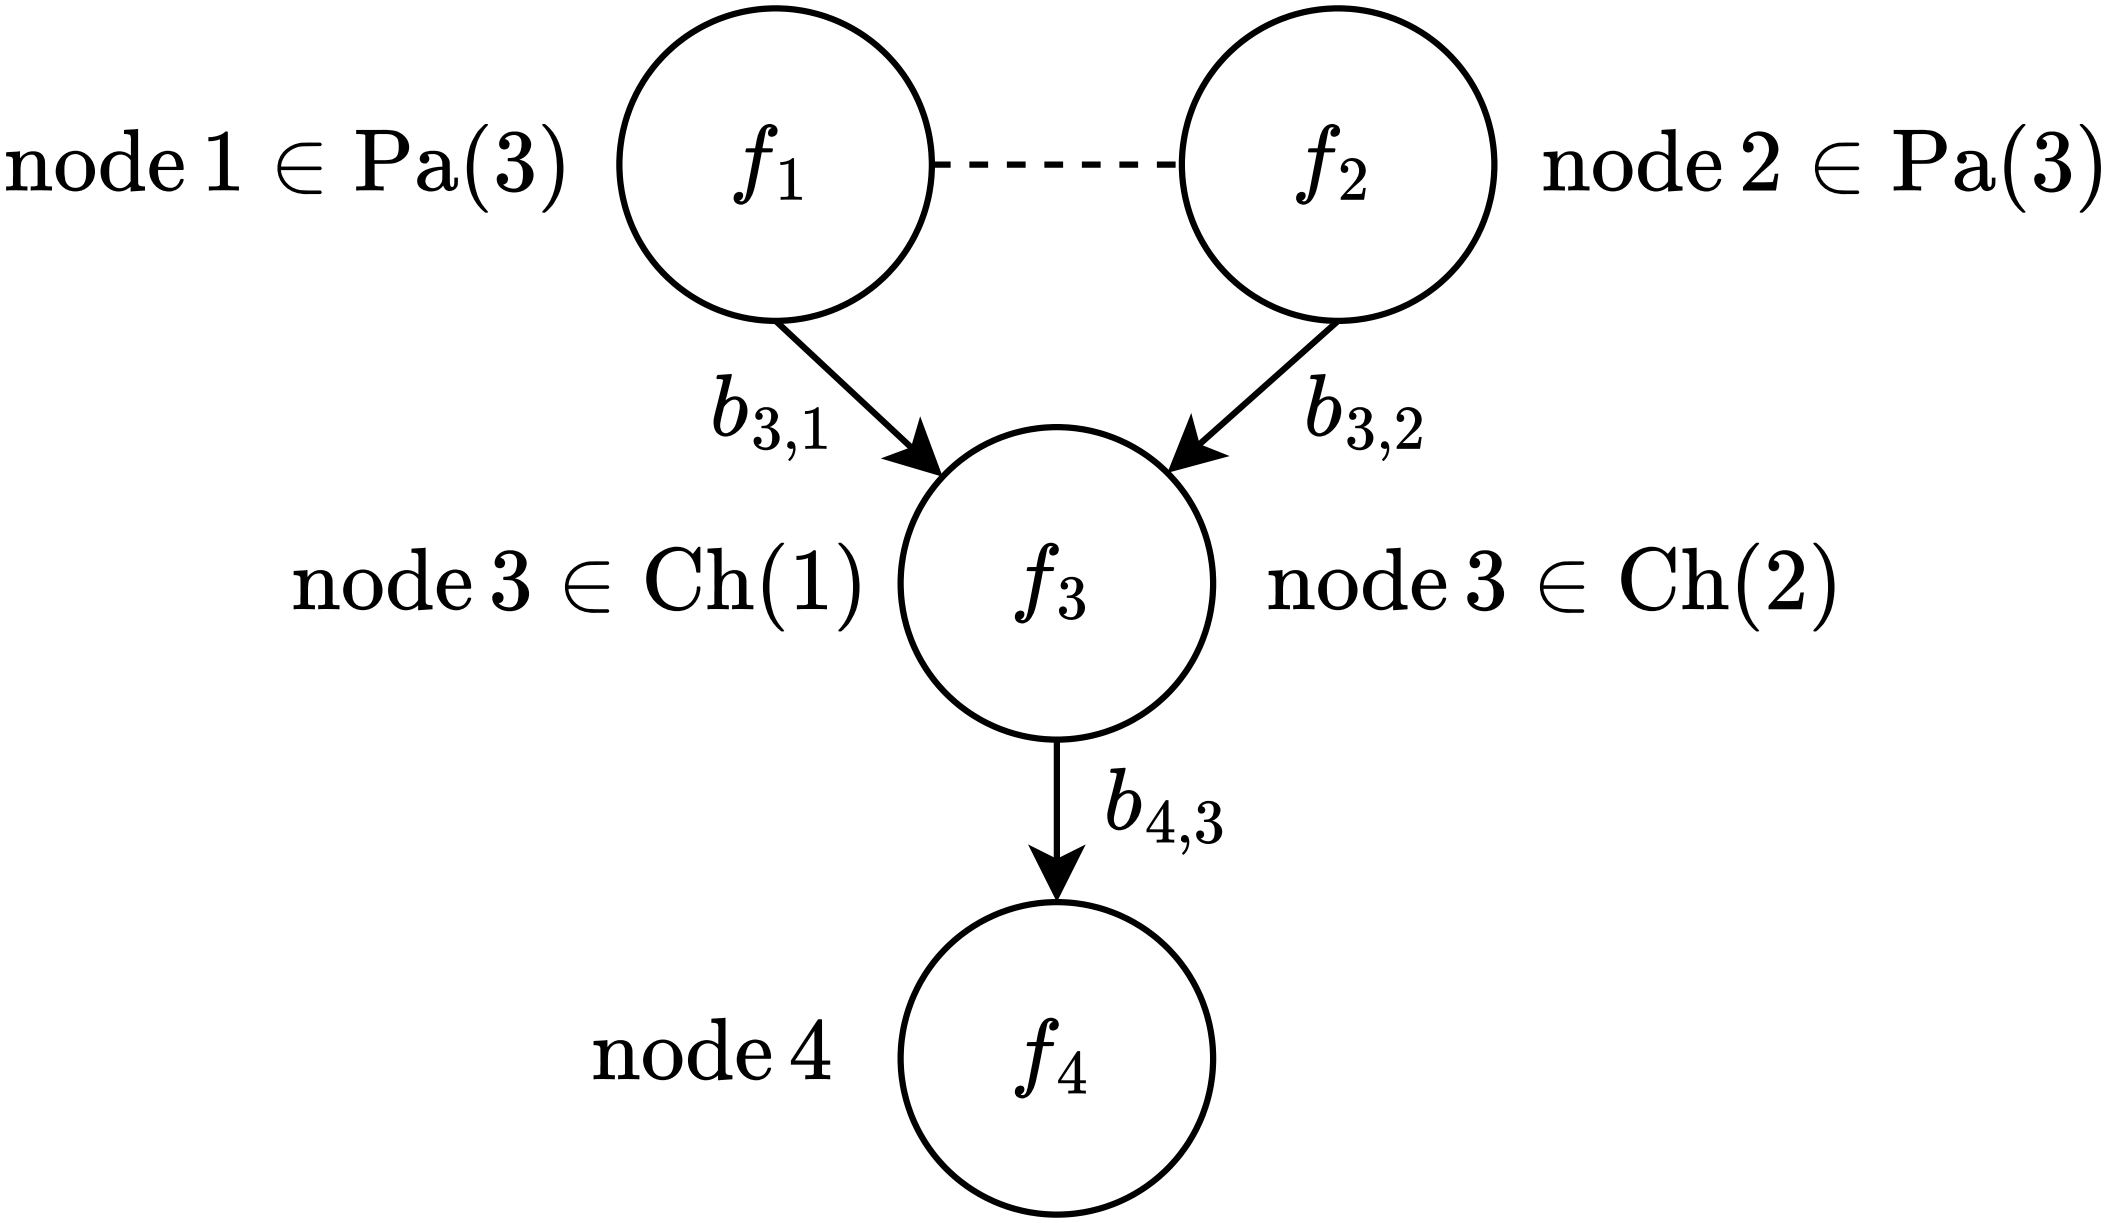
\includegraphics[scale=0.85]{Fig6.png}
	\caption{Illustration of the $K$-step look-ahead problem. The node $\mathcal{D}^0$ represents the data we observed so far, and the node $\bf x$ is the design point we are finding.}
	\label{Fig6}
\end{figure*}
%============================================================

\subsubsection{Multi-step look-ahead acquisition functions}\label{Sec612}

Despite their simplicity and computational efficiency, one-step look-ahead acquisition functions tend to prefer exploitation over exploration~\citep{Hennig2022}.
To mitigate this limitation, multi-step look-ahead (or non-myopic) acquisition functions have been developed.
These acquisition functions excel by considering the impact of future selections on the decision of next design points~\citep{Streltsov1999,Ginsbourger2010,Gonzalez2016,Lam2016,JWu2019,Jiang2020}.
However, it still remains challenging to handle an exact multi-step look-ahead problem as we have to marginalize uncertain objective function value and design point location in each step~\citep{Gonzalez2016,Hennig2022}.
What we can expect is to use either
two-step look-ahead acquisition functions via Monte-Carlo estimation~\citep{JWu2019} or multi-step look-ahead acquisition functions via approximation techniques, such as rollout~\citep{Lam2016,Lee2020,Paulson2022}, GLASSES~\citep{Gonzalez2016}, and multi-step~\citep{Jiang2020}.
In the following, we briefly describe some multi-step look-ahead acquisition functions.
For the detailed implementation, the reader is encouraged to refer to the corresponding references.

Figure~\ref{Fig6} describes BO as a multistage decision problem for finding ${\bf x},{\bf x}^2,\dots,{\bf x}^{K}$.
Our current objective is to determine $\bf x$ based on the information available in the observed data $\mathcal{D}^0$.
This decision is influenced by the choices we make for future selections ${\bf x}^2,\dots,{\bf x}^{K}$.

For any data $\mathcal{D}$, we define
% Equation 53
\begin{equation}\label{Eq53}
	u(\mathcal{D}) = \underset{({\bf x},f_{\text{H}}) \in \mathcal{D}}{\min}\,f_{\text{H}}({\bf x}),
\end{equation} 
which returns the best solution found among the elements of $\mathcal{D}$.
Based on $u(\cdot)$, we can further define the one-step look-ahead acquisition function $\alpha_1({\bf x}|\mathcal{D})$ as
% Equation 54
\begin{equation}\label{Eq54}
	\begin{aligned}
	&\alpha_1({\bf x}|\mathcal{D})\\
	&=\mathbb{E}_{f_\text{H}}\left[\max\left(u(\mathcal{D}) - u(\mathcal{D} \cup ({\bf x},f_\text{H}({\bf x})),0\right)
	|{\bf x},\mathcal{D}\right],
	\end{aligned}
\end{equation} 
which is EI given in Eq~(\ref{Eq43}).

The Bellman's principle of optimality allows the computation of the $K$-step look-ahead acquisition function recursively, such that
% Equation 55
\begin{equation}\label{Eq55}
	\begin{aligned}
	&\alpha_K({\bf x}|\mathcal{D})\\
	& =\alpha_1({\bf x}|\mathcal{D}) + \mathbb{E}_{f_\text{H}}\left[\underset{\bf x'}{\max}\,\alpha_{K-1}({\bf x}'|\mathcal{D} \cup ({\bf x},f_\text{H}({\bf x}))\right],
\end{aligned}
\end{equation}
where $\alpha_K(\cdot)$ and $\alpha_{K-1}(\cdot)$ represent the $K$- and $(K-1)$-step look-ahead acquisition functions, respectively.

Using Eq.~(\ref{Eq55}), \cite{Jiang2020} proposed the following $K$-step look-ahead acquisition function for the representation in Fig.~\ref{Fig6}:
% Equation 56
\begin{equation}\label{Eq56}
	\begin{aligned}
		\alpha_K({\bf x}|\mathcal{D}^0) & =\alpha_1({\bf x}|\mathcal{D}^0) + \mathbb{E}_{f_\text{H}}\left[\underset{\bf x'}{\max}\,\alpha_{K-1}({\bf x}'|\mathcal{D}^1)\right] \\
		& = \alpha_1({\bf x}|\mathcal{D}^0) +\mathbb{E}_{f_\text{H}}\Bigg[\underset{{\bf x}^2}{\max}\,\Big(\alpha_1({{\bf x}}^2|\mathcal{D}^1) + \\
		& \quad \mathbb{E}_{f_\text{H}^2}\Big[\underset{{\bf x}^3}{\max}\,\alpha_1({\bf x}^3|\mathcal{D}^2)+\dots  \Bigg].
	\end{aligned}
\end{equation}

\cite{JWu2019} proposed two-step look-ahead acquisition function $\alpha_2({\bf x}|\mathcal{D}^0)$ that, via the Monte-Carlo simulation, can be computationally efficient.
$\alpha_2({\bf x}|\mathcal{D}^0)$ reads
% Equation 57
\begin{equation}\label{Eq57}
		\alpha_2({\bf x}|\mathcal{D}^0) =\alpha_1({\bf x}|\mathcal{D}^0) + \mathbb{E}_{f_\text{H}}\left[\underset{{\bf x}^2}{\max}\,\alpha_1({\bf x}^2|\mathcal{D}^1)\right].
\end{equation}

\cite{Gonzalez2016} introduced GLASSES acquisition function by assuming a joint PDF of the future selections from which a batch of design points can be generated in each iteration.
Accordingly, GLASSES reads
% Equation 58
\begin{equation}\label{Eq58}
		\alpha_K({\bf x}|\mathcal{D}^0) \approx \alpha_1({\bf x}|\mathcal{D}^0) + \mathbb{E}_{f_\text{H}}\left[\Lambda_{K-1}(\textbf{X}_\text{x}|\mathcal{D}^1)\right],
\end{equation}
where 
$\textbf{X}_\text{x} \in \mathbb{R}^{(K-1) \times d}$ is a fixed matrix whose rows are the future design points ${\bf x}^2,\dots,{\bf x}^K$. $\Lambda_{K-1}(\textbf{X}_\text{x}|\mathcal{D}^1)$ is a batch value function for the matrix  $\textbf{X}_\text{x}$ given the unknown data $\mathcal{D}^1$, such that 
% Equation 59
\begin{equation}\label{Eq59}
	\begin{aligned}
	& \Lambda_{K-1}(\textbf{X}_\text{x}|\mathcal{D}^1) =\mathbb{E}_{f_\text{H}^2,\dots,f_\text{H}^K}\Bigg[\max\Big(u(\mathcal{D}^1)\\
	& -u( \mathcal{D}^1 \cup  ({\bf x}^2,f_\text{H}^2) \cup \cdots \cup  ({\bf x}^K,f_\text{H}^K) \Big)|\textbf{X}_\text{x},\mathcal{D}^1\Bigg].
	\end{aligned}
\end{equation}

Alternatively, rollout strategies~\citep{Lam2016,Lee2020,Paulson2022} formulate the selection of new design points as a Markov
decision process.
Thus, the multi-step look-ahead acquisition function is the expected total reward of this Markov
decision process.
Then, the maximum of such reward can be found by dynamic programming~\citep{Rao2019}.
%============================================================

\begin{algorithm}
	\caption{Pseudo-code for MF BO using without-fidelity-consideration acquisition function.}\label{Algo3}
	\begin{algorithmic}[1]
		\State \textbf{Input:} $\mathcal{X}$, $K$, $\mathcal{D}_t$ $(t=1,\dots,T)$;
		\State $\mathcal{D}^0 \gets \mathcal{D}_1 \cup \dots \cup \mathcal{D}_T$;
		\State $({\bf x}_{\min},f_{\min}) \gets u(\mathcal{D}^0)$;
		
		\For {$k=1:K$} 
		\State Construct MF emulator $\hat{f}_\text{H}^k({\bf x})$;
		\State Formulate MF acquisition function $\alpha({\bf x})$;
		\State ${\bf x}^{k} \gets \underset{{\bf x}}{\mathrm{argmax}} \ \ \alpha({\bf x})$ s.t. ${\bf x} \in \mathcal{X}$;
		\State $\mathcal{D}_t \gets \mathcal{D}_t \cup ({\bf x}^{k},f_t({\bf x}^{k}))$ $(t=1,\dots,T)$;
		\State $\mathcal{D}^k \gets \mathcal{D}_1 \cup \dots \cup \mathcal{D}_T$;
		\State $({\bf x}_{\min},f_{\min}) \gets u(\mathcal{D}^k)$;
		\EndFor
		
		\State \Return $({\bf x}_{\min},f_{\min})$.
	\end{algorithmic}
\end{algorithm}

\begin{algorithm}
	\caption{Pseudo-code for MF BO using heuristic approach.}\label{Algo4}
	\begin{algorithmic}[1]
		\State \textbf{Input:} $\mathcal{X}$, $K$, $\mathcal{D}_t$ $(t=1,\dots,T)$;
		\State $\mathcal{D}^0 \gets \mathcal{D}_1 \cup \dots \cup \mathcal{D}_T$;
		\State $({\bf x}_{\min},f_{\min}) \gets u(\mathcal{D}^0)$;
		
		\For {$k=1:K$} 
		\State Construct MF emulator $\hat{f}_\text{H}^k({\bf x})$;
		\State Formulate MF acquisition function $\alpha({\bf x},t)$;
		
		\For {$t=1:T$} 
		\State $({\bf x}_t^{k},t,\alpha^k) \gets {\min }\ \ \alpha({\bf x},t)$ s.t. ${\bf x} \in \mathcal{X}$;
		\EndFor
		
		\State $({\bf x}^{k},t) \gets\max\{\alpha^k,\, t=1,\dots, T\}$
		\State $\mathcal{D}_t \gets \mathcal{D}_t \cup ({\bf x}^{k},f_t({\bf x}^{k}))$;
		\State $\mathcal{D}^k \gets \mathcal{D}_1 \cup \dots \cup \mathcal{D}_T$;
		\State $({\bf x}_{\min},f_{\min}) \gets u(\mathcal{D}^k)$;
		\EndFor
		
		\State \Return $({\bf x}_{\min},f_{\min})$.
	\end{algorithmic}
\end{algorithm}


\begin{algorithm}
	\caption{Pseudo-code for MF BO using sequential selection approach.}\label{Algo5}
	\begin{algorithmic}[1]
		\State \textbf{Input:} $\mathcal{X}$, $K$, $\mathcal{D}_t$ $(t=1,\dots,T)$;
		\State $\mathcal{D}^0 \gets \mathcal{D}_1 \cup \dots \cup \mathcal{D}_T$;
		\State $({\bf x}_{\min},f_{\min}) \gets u(\mathcal{D}^0)$;
		
		\For {$k=1:K$} 
		\State Construct MF emulator $\hat{f}_\text{H}^k({\bf x})$;
		\State Formulate MF acquisition function $\alpha({\bf x})$;
		\State ${\bf x}^{k} \gets \underset{{\bf x}}{\mathrm{argmax}} \ \ \alpha({\bf x})$ s.t. ${\bf x} \in \mathcal{X}$;
		\State Formulate fidelity-query function $\gamma({\bf x}^{k},t)$;
		\State $t \gets \underset{t}{\mathrm{argmax}} \ \ \gamma({\bf x}^{k},t)$ s.t. $t \in \{1,\dots,T\}$;
		\State $\mathcal{D}_t \gets \mathcal{D}_t \cup ({\bf x}^{k},f_t({\bf x}^{k}))$;
		\State $\mathcal{D}^k \gets \mathcal{D}_1 \cup \dots \cup \mathcal{D}_T$;
		\State $({\bf x}_{\min},f_{\min}) \gets u(\mathcal{D}^k)$;
		\EndFor
		
		\State \Return $({\bf x}_{\min},f_{\min})$.
	\end{algorithmic}
\end{algorithm}
%============================================================

\subsection{Acquisition functions considering fidelities}\label{Sec62}

In MF BO, we replace $\hat{f}_\text{H}^k(\cdot)$ in Step~10 of Algorithm~\ref{Algo1} with one of the GP-based emulators described in Section~\ref{Sec6}.
This raises a question of how to incorporate the information about fidelities, i.e., $t \in \{1,\dots,T\}$, into the acquisition function so that we can select a new design point and an appropriate simulation for computing the corresponding objective function value. 
 
The use of different MF emulators and/or different acquisition functions of generic BO leads to the variety of MF acquisition functions. Nevertheless, we can categorize the MF acquisition functions into the following three groups: 
\begin{itemize}
	\item Without-fidelity consideration (Algorithm~~\ref{Algo3}).
	
	\item Heuristic approach (Algorithm~~\ref{Algo4}).
	
	\item Sequential selection (Algorithm~~\ref{Algo5}).
	 
\end{itemize}

\textbf{Without-fidelity consideration}.
The acquisition function only depends on design variables $\bf x$.
Once the new design point ${\bf x}^k$ has been found, we have to carry out $T$ simulations associated with all $T$ fidelities for updating the MF emulator.
Algorithm~\ref{Algo3} shows the pseudo-code for MF BO using this approach.
In Step 7 of Algorithm~\ref{Algo3}, \cite{Forrester2007} used EI in which $f_{\min}$ was selected from the highest fidelity. \cite{Perdikaris2016} also adopted EI but $f_{\min}$ was the best value among those from all fidelities.
This approach may show its advantages if the computational cost of all LF samples can compensate for the difference between the total cost of all HF samples when using the highest-fidelity emulator only and that when using the MF emulator.

\textbf{Heuristic approach}.
The acquisition function depends on both $\bf x$ and $t$.
This acquisition function is often derived by modifying one of the one-step look-ahead acquisition functions of generic BO using some auxiliary functions to consider the computational cost of each fidelity level and/or how the simulation associated with the new design point from each fidelity affects the accuracy improvement of the MF emulator.
Algorithm~\ref{Algo4} shows the pseudo-code for MF BO using this approach.
In Steps 7--10 of Algorithm~\ref{Algo4}, a new design point ${\bf x}^k$ can be found for each enumerated value of $t$, and the pair of $t$ and ${\bf x}^k$ that provides the best acquisition function value is selected.
Due to its simplicity, the heuristic approach has been widely employed in engineering design~\citep{Huang2006,Poloczek2017,YZhang2018,Ghoreishi2019,Ruan2020,Shu2021,Fiore2021,Sacher2021,He2021,Huang2023,Ribeiro2023,Winter2023,Foumani2023,Grassi2023,Fiore2023}.

\textbf{Sequential selection}.
This approach consists of two steps: (i) select the new design point ${\bf x}^k$ and (ii) select the fidelity $t$ with ${\bf x}^k$ found in step (i)~\citep{Chen2016,Kandasamy2017,Meliani2019,Tran2020a,Tran2020b,Kandasamy2019}.
The main difference between this approach and the heuristic approach is that the selection of ${\bf x}^k$ is independent of $t$.
This means the solution improvement is separated from the consideration of computational cost and the prediction improvement of the MF emulator.
Algorithm~\ref{Algo5} shows the pseudo-code for MF BO using the sequential approach. 

In the following, we briefly describe some methods of the heuristic and sequential selection approaches.

Let $\mu^k_{f_\text{H}}(\cdot)$ and $\sigma_{f_\text{H}}^{2,k}(\cdot)$ denote the mean and variance of the MF emulator $\hat{f}_\text{H}^k(\cdot)$.
Let $c_1,\dots,c_T$ denote the computational costs associated with the simulations of $1,\dots,T$ fidelities, respectively.

One of the first heuristic acquisition functions by \cite{Huang2006} is the product of the so-called augmented EI (AEI)~\citep{Huang2006a}, developed for generic BO with noisy objective functions, and two auxiliary terms for considering the fidelity levels $\alpha_1({\bf x},t)$ and $\alpha_2(t)$.
This acquisition function reads
\begin{equation}
		\alpha({\bf x},t) = \text{AEI}({\bf x}) \alpha_1({\bf x},t) \alpha_2(t).
\end{equation}
Here $\alpha_1({\bf x},t)$ is the correlation between the posterior estimate at $\bf x$ of emulator $t$ and that of emulator $T$.
Since $\alpha_1 = 1$ when $t=T$, $\alpha_1$ tends to promote high fidelities. 
Meanwhile, $\alpha_2(t) = c_T/c_t$ is the ratio between the computational cost per simulation on the highest fidelity $T$ and that on the fidelity $t$.
In contrast to $\alpha_1$, $\alpha_2$ favors low fidelities.

Extensions of Eq.~(\ref{Eq60}) are problem-dependent.
The standard deviation constituting $\text{AEI}({\bf x})$, which only depends on ${\bf x}$, has been modified as a function of both ${\bf x}$ and $t$, given that only two fidelity levels are considered~\citep{YZhang2018,Fiore2021,Ruan2020,Grassi2023}.
In addition to modifying $\text{AEI}({\bf x})$, different forms of $\alpha_1({\bf x},t)$ has been developed.
For example, \cite{Sacher2021} used $\alpha_1({\bf x},t) = \max\left(0,1-\sigma_{f_\text{H}}^{2,k+1}({\bf x}|{\bf x},t)/\sigma_{f_\text{H}}^{2,k}({\bf x})\right)$, where $\sigma_{f_\text{H}}^{2,k+1}({\bf x}|{\bf x},t)$ is the posterior variance of the updated MF emulator with the new sampling point generated by simulation $t$.
This $\alpha_1({\bf x},t)$ also favors high fidelities from which the new sampling points tend to reduce the prediction error.
\cite{Huang2023} defined $\alpha_1({\bf x},t)$ as the Kullback–Leibler divergence of two posterior GPs associated with two fidelity levels.   
Furthermore, other authors formulated the MF acquisition function as the ratio between an acquisition function of generic BO and the computational cost per simulation on the fidelity~\citep{Ghoreishi2019,Winter2023,Foumani2023}.
Some authors have started examining the empirical performance of two-step look-ahead MF EIs~\citep{Ghoreishi2019,Fiore2023} because most heuristic MF acquisition functions are one-step look-ahead.

As a method of the sequential approach, \cite{Chen2016}, after finding ${\bf x}^k$ by maximizing EI, formulated a fidelity-query function $\gamma({\bf x}^k,t)$ (Step 8 of Algorithm~\ref{Algo5}) using the so-called preposterior analysis.
The preposterior analysis was to examine how the standard deviation of the MF emulator at ${\bf x}^k$ reduces when fictitious simulation data for each fidelity are added to the current real training data.
Here, due to the use of auto-regressive approach, the fictitious simulation data for fidelity $t$ at ${\bf x}^k$ consisted of the samples generated from a Gaussian characterized by the mean and variance at ${\bf x}^k$.
In this way, the reduction of standard deviation associated with fidelity $t$ was defined as $\sigma_{f_\text{H}}^k({\bf x}^k)-\bar{\sigma}({\bf x}^k,t)$, where $\bar{\sigma}({\bf x}^k,t)$ is the expected standard deviation of the updated GP posterior after the fictitious simulation data for fidelity $t$ are added to the current real training data several times.
By further considering the computational cost per simulation on the fidelity, \cite{Chen2016} defined the fidelity-query function as
% Equation 61
\begin{equation}\label{Eq61}
		\gamma({\bf x}^k,t) = \frac{\sigma_{f_\text{H}}^k({\bf x}^k)-\bar{\sigma}({\bf x}^k,t)}{\sigma_{f_\text{H}}^k({\bf x}^k)-\bar{\sigma}({\bf x}^k,T)} \frac{c_T}{c_t}.
\end{equation}
A large value of $\gamma({\bf x}^k,t)$ indicates a large reduction in prediction uncertainty per unit of computational cost at $({\bf x}^k,t)$.
A similar fidelity-query function can be found in~\cite{Tran2020a,Tran2020b}.

\cite{Kandasamy2017} defined $\gamma({\bf x}^k,t)$ as the negative value of the computational cost per simulation on the fidelity.
They also imposed two constraints on the maximization of $\gamma({\bf x}^k,t)$.
The first constraint says that the posterior variance associated with $({\bf x}^k,t)$ should be larger than a pre-specified threshold value, which tends to promote exploration.
Meanwhile, the second constraint says that we should find the maximizer of $\gamma({\bf x}^k,t)$ in a neighborhood of $T$ that can shrink over time.
This means, we eventually find a point that is close to $T$. 
In this context, the constraints in Step 9 of Algorithm~\ref{Algo5} should consist of the aforementioned two constraints and a bound constraint on $t$ as $t$ is considered as a continuous variable~\citep{Kandasamy2017} (see Section~\ref{Sec561}).

Alternatively, \cite{Meliani2019} formulated $\gamma({\bf x}^k,t)$ by drawing from the idea that the use of LF simulations favors exploration, and that of HF ones favors exploitation.
Therefore, multiple fidelities can be used simultaneously.
In particular, $\gamma({\bf x}^k,t)$ was defined as the ratio between the total uncertainty reduction when adding the new data from simulations whose fidelities are not greater than $t$ and the total computational cost of these simulations.
As a result, the simulations whose fidelities are not greater than $t$ were called in Step 10 of Algorithm~\ref{Algo5}, which differs from other methods of the sequential approach.
Note that this method belongs to the without-fidelity consideration approach when $t=T$.
%============================================================

\subsection{Maximization of acquisition functions}\label{Sec63}

Because it is difficult to examine the convexity of most acquisition functions presented in Sections~\ref{Sec61} and \ref{Sec62}, it is possible to obtain different values of ${\bf x}^k$ after maximizing $\alpha({\bf x})$ or $\alpha({\bf x},t)$. 
Thus, it is preferable to maximize these acquisition functions using a global optimization algorithm.
However, it may be useful to discretize the design variable space or use a sampling method when maximizing an information-based acquisition function.
In Table~\ref{Table5}, we list optimization algorithms used to maximize several acquisition functions.

% Table 5 
\begin{table*}
	\caption{Summary of optimization algorithms for maximizing acquisition functions.}
	\label{Table5}
	\centering
	\begin{tabularx}{\textwidth}{lXX}
		\hline \noalign{\smallskip}
 		Acquisition function & Optimization algorithm & Reference\\
		\hline \noalign{\smallskip}
		
		 EI and its variants & Branch-and-bound algorithm & \cite{Jones1998}\\
		 \noalign{\smallskip}
		 & Nelder-Mead simplex method & \cite{Huang2006,Huang2006a}\\
		 \noalign{\smallskip}
		 & Genetic algorithm (GA) & \cite{Forrester2007,Chen2016,YZhang2018,Bailly2019,Do2022}\\
		 \noalign{\smallskip}
		 & Particle swarm optimization & \cite{Kontogiannis2020b,Ribeiro2023}\\
		 \noalign{\smallskip}
		 & Limited-memory  Broyden-Fletcher-Goldfarb-Shanno (L-BFGS) & \cite{Frazier2018,Bonfiglio2018b}\\
		 \noalign{\smallskip}
		 & BFGS & \cite{Sobester2005}\\
		 \noalign{\smallskip}
		 & Discretizing design variable space & \cite{Ghoreishi2019,Grassi2023}\\
		 \noalign{\smallskip}
		 & Covariance matrix adaptation evolution strategy & \cite{Tran2020a,Tran2020b}\\
		\noalign{\smallskip}
		
		GP-UCB and its variants & Direct optimization algorithm & \cite{Kandasamy2016,Kandasamy2017}\\
		\noalign{\smallskip}
		
		PI and its variants & GA & \cite{Ruan2020}\\
		\noalign{\smallskip}
		
		KG & Multi-start stochastic gradient& \cite{JWu2016}\\
		\noalign{\smallskip}
		
		IAGO & Discretizing design variable space & \cite{Villemonteix2009}\\
		\noalign{\smallskip}
		
		ES & Sampling combined with L-BFGS & \cite{Hennig2012}\\
		\noalign{\smallskip}
		
		PES & Sampling combined with either a local search or Nelder-Mead simplex method& \cite{Lobato2014}\\
		\noalign{\smallskip}
		
		MES & Sampling combined with either a local search or Nelder-Mead simplex method& \cite{ZWang2017}\\
		\hline \noalign{\smallskip}
		
	\end{tabularx}
\end{table*}
%============================================================

\subsection{Portfolio of acquisition functions}\label{Sec64}

No acquisition function works well on all problems of interest as the preferred search strategy may vary during different phases of a sequential optimization process ~\citep{Shahriari2016}.
A promising solution to address this issue involves employing a portfolio of multiple acquisition functions~\citep{Hoffman2014,Shahriari2014}.
The rationale behind this approach is to leverage the interaction between different acquisition functions to safeguard against the potential failure of any single search strategy.
This collaborative interaction is quantified via a unified portfolio metric, which can take the form of a meta-criterion~\citep{Hoffman2014} or an entropy search metric~\citep{Shahriari2014}.
The approach then requires two steps.
First, it finds a collection of new design points by maximizing each individual acquisition function within the portfolio.
Second, from this set of design points, it selects the actual design point that maximizes the portfolio metric.
%============================================================

% Section 7
\section{Further research topics}\label{Sec7}

Recent advances in BO have focused on solving intricate optimization problems, which stem from the nature of the problems or from the inherent limitation of BO~\citep{Wang2023}.  
Some of these problems include constrained optimization, high-dimensional optimization, optimization under uncertainty, multi-objective optimization, and combinatorial optimization.  
In this section, we review some extensions of BO to address these problems.
By doing so, we expect to shed light on potential opportunities for future research in the realm of MF BO.
%============================================================
\subsection{Constrained optimization}\label{Sec71}

Constrained BO handles the following problem:
% Equation 62
\begin{equation}\label{Eq62}
	\begin{aligned}
		\underset{{\bf x} \in \mathcal{X}}{\min} \ \ & f_\text{H}(\bf x)\\
		\textrm{s.t.} \ \ 
		& g_{\text{H},i}({\bf x}) \leq 0,\ \ i=1,\dots,I, 
	\end{aligned}
\end{equation}
where $g_{\text{H},i}({\bf x})$ are expensive-to-compute constraint functions evaluated via costly simulations.
We also assume that $g_{\text{H},i}({\bf x})$ are conditionally independent.

To solve problem~(\ref{Eq62}) via BO, \cite{Schonlau1998} proposed a constrained EI (CEI) acquisition function.
CEI is the product of EI in Eq.~(\ref{Eq43}) and the probability that all inequality constraints are satisfied (i.e., probability of feasibility).
Accordingly, CEI reads
% Equation 63
\begin{equation}\label{Eq63}
	\alpha_\text{c}({\bf x}) = \text{EI}({\bf x}) \mathbb{P}[\hat{g}_{\text{H},1}({\bf x}) \leq 0,\dots,\hat{g}_{\text{H},I}({\bf x}) \leq 0],
\end{equation}
where $\hat{g}_{\text{H},i}({\bf x})$, $i=1,\dots,I$, is the GP posterior of $g_{\text{H},i}({\bf x})$.

The probability of feasibility $\mathbb{P}[\hat{g}_{\text{H},1}({\bf x}) \leq 0,\dots,\hat{g}_{\text{H},I}({\bf x}) \leq 0]$ transfers the constrained optimization problem to an unconstrained problem by penalizing unfeasible regions.
As a consequence, it may put more weight on the feasible regions associated with a large safety margin and overlook the boundary of feasible space on which the optimal solution is often located.

Since $\hat{g}_{\text{H},i}({\bf x})$ are conditionally independent, CEI becomes
% Equation 64
\begin{equation}\label{Eq64}
	\alpha_\text{c}({\bf x}) = \text{EI}({\bf x}) \prod_{i=1}^I\Phi\left(\frac{-\mu_{\text{g},i}^k({\bf x})}{\sigma_{\text{g},i}({\bf x})}\right)
\end{equation}
where $\mu_{\text{g},i}$ and $\sigma_{\text{g},i}$ are the mean and standard deviation of $\hat{g}_{\text{H},i}({\bf x})$, respectively.

Note that it is not necessary to formulate $\alpha_\text{c}({\bf x})$ if $g_{\text{H},i}({\bf x})$ is easy-to-compute.
In this case, we can simply maximize any unconstrained acquisition functions in Section~\ref{Sec61} subject to these constraints.

The performance of CEI has been tested by~\cite{Gardner2014,Sobester2014,Kontogiannis2020b}.
In addition, MF-BO has recently incorporated the probability of feasibility or its modifications into a heuristic MF acquisition function to address engineering optimization problems~\citep{Ghoreishi2019,Ruan2020,Ribeiro2023}.
However, decoupling the selection of a new design point and the selection of fidelity level for constrained optimization is still an open issue.

\cite{Gramacy2011} introduced the concept of integrated expected conditional improvement (IECI) for solving problem~(\ref{Eq62}) with inexpensive constraint functions.
This concept was then extended to solve problems featuring expensive constraint functions.
IECI reads
% Equation 65
\begin{equation}\label{Eq65}
	\alpha_\text{c}({\bf x}) = \int_{\mathcal{X}} \left[\text{EI}({\bf x'}) - \text{EI}({\bf x'}|{\bf x})\right] p({\bf x'}) \text{d}{\bf x'},
\end{equation}
where $\text{EI}({\bf x'})$ is the expected improvement at $\bf x'$, $\text{EI}({\bf x'}|{\bf x})$ is the expected improvement at $\bf x'$ given that $\left({\bf x},f_\text{H}({\bf x})\right)$ is added to the data, and $p({\bf x'})$ is the PDF of ${\bf x'}$.

We see that IECI handles the constraints via $p({\bf x'})$, which may be uniform for feasible ${\bf x'} \in \mathcal{X}$ and zero otherwise.
When the constraint functions are costly, $p({\bf x'})$ can be approximated by performing Monte-Carlo simulation on the surrogates of these functions~\citep{Gramacy2011}.
IECI also allows the selection of new design points that violate the constraints at cost of useful information about the function.
The following considerations should be taken into account if one wishes to use IECI for MF BO: (i) how to incorporate the fidelity level into approximation of $p({\bf x'})$ and (ii) how to select the fidelity level if an infeasible design is found after maximizing $\alpha_\text{c}({\bf x})$.  

Alternative, \cite{Gramacy2016} adopted BO to minimize the augmented Lagrangian of problem~(\ref{Eq62}), which reads
% Equation 66
\begin{equation}\label{Eq66}
	\begin{aligned}
	 	\mathcal{L}({\bf x}|\lambda_1,\dots,\lambda_I,\rho_0) & = f_\text{H}({\bf x}) + \sum_{i=1}^{I} \lambda_i g_{\text{H},i}({\bf x}) \\
	 	& + \frac{1}{2 \rho_0} \sum_{i=1}^{I} \max(0,g_{\text{H},i}({\bf x})), 
	\end{aligned} 
\end{equation}
where  $\rho_0>0$ is the penalty parameter and $\lambda_1 \geq 0,\dots,\lambda_I \geq 0$ are Lagrange multipliers associated with the inequality constraint functions.

The augmented Lagrangian method starts by assigning initial values of $\rho_0$ and $\boldsymbol{\lambda}=[\lambda_1 \geq 0,\dots,\lambda_I]^\intercal$.
It then sequentially finds the minimizer of the augmented Lagrangian corresponding to these values, and updates $\rho_0$ and $\boldsymbol{\lambda}$ for the next iterate with the obtained minimizer.

In the BO setting, the idea is to construct in each iterate a GP model for $\mathcal{L}$ based on its observations for several samples of $\rho_0$, $\boldsymbol{\lambda}$, design variable vectors, and the corresponding values of the objective and constraint functions.
Then, the next design point is found by maximizing the EI acquisition function, and the new parameters $\rho_0$ and $\boldsymbol{\lambda}$ are updated accordingly. 

The expected volume minimization (EVM) by ~\cite{Picheny2014} is another acquisition function for constrained BO.
By integrating the product of the probability of improvement and the probability of feasibility, EVM is defined as
% Equation 67
\begin{equation}\label{Eq67}          
	\begin{aligned}
		\alpha_\text{c}({\bf x}) & = \int_{\mathcal{X}} \mathbb{P}\left[f_\text{H}({\bf x}) \leq \min(f_\text{H}({\bf x}),f_{\min})\right]\\ 
		& \qquad \mathbb{P}[g_{\text{H},1}({\bf x}) \leq 0,\dots,g_{\text{H},I}({\bf x}) \leq 0] \text{d}{\bf x}  \\
		& + \int_{\mathcal{X}} \mathbb{P}\left[f_\text{H}({\bf x}) \leq f_{\min}\right]\\
		& \qquad \left(1-\mathbb{P}[g_{\text{H},1}({\bf x}) \leq 0,\dots,g_{\text{H},I}({\bf x}) \leq 0]\right) \text{d}{\bf x}.
	\end{aligned} 
\end{equation}
%where $f_{\min}$ is the best value of the objective found so far.
The first and second integrals correspond to the probability of improvements considering the feasibility and unfeasibility of the new design point, respectively.
In general, maximizing EVM is costly as it requires the use of numerical integration over $\mathcal{X}$.
%============================================================

\subsection{High-dimensional optimization}\label{Sec72}

The size of a problem is a measure of its complexity.
Thus, it is reasonable to classify optimization problems into three classes~\citep{Luenberger2008}: 
\begin{itemize}
	\item Small-dimensional problems, which have about five a fewer design variables and constraints.
	
	\item Medium-dimensional problems, which have from about five to a thousand design variables and constraints.
	
	\item High-dimensional problems, which have thousands or even millions of variables and constraints.
\end{itemize}
While this classification is not rigid, it reflects not only the size but also the fundamental differences in solution approach associated with varying problem sizes~\citep{Luenberger2008}.

It is of great practical and theoretical interest to extend the BO framework to high-dimensional optimization problems, thanks to its efficiency in solving problems of less than 20 design variables~\citep{Frazier2018}.
However, this faces two computational challenges.
First, the global GP scales cubically with the number of training data points~\citep{Rasmussen2006,Snoek2015}, which is proportional to the number of design variables.
Second, maximizing a high-dimensional acquisition function is nontrivial because it is mostly flat at high dimension~\citep{Rana2017}.
These two challenges make high-dimensional BO is related to, but distinct from scalable GP modeling approaches~\citep{HLiu2020}. 


Recent advances in high-dimensional BO follow three main approaches~\citep{Daulton2022a}: 
\begin{itemize}
	\item Exploiting low, active/effective dimensional subspace of the design variables.
	
	\item Exploiting the additive structures of the objective and/or constraint functions.
	
	\item Trust-region BO.
\end{itemize}
The first approach constructs the functions in an unknown low-dimensional subspace of the design variables, and then performs BO in this subspace instead of in the high-dimensional space~\citep{ZWang2016,Nayebi2019,Munteanu2019,Letham2020}.
Methods of this approach differ in the way of defining the low-dimensional subspace.
The second approach relies on the decomposition of the objective/constraint functions into some partitioning of dimensions, so that the global GPs can be written as a sum of several GPs in small, disjoint groups of dimensions~\citep{Kandasamy2015,Gardner2017,ZWang2018}.
The obstacle of this approach is to decide the way to partition the design variable space and the observed data. 
The third approach performs BO using independent local GPs constructed from multiple trust regions to avoid over-exploration~\citep{Eriksson2019,Eriksson2021,Daulton2022a}.
The focus of this approach is on updating both the size of trust regions and the independent local GPs.

\noindent
\textbf{Subspace-based approach}.

Sensitivity analysis~\citep{Spagnol2019} is a classical method of the subspace-based approach that selects the most-contributing design variables and ignores the less-contributing ones.
A drawback of this method is that it cannot capture the models varying most prominently along the directions that are not aligned with the original coordinate system of the design variable space~\citep{Constantine2014}, leading to the quest for active/effective subspace.

A random linear embedding~\citep{ZWang2016} is one of the important methods of the subspace-based approach.
It states that for any design variable vector ${\bf x} \in \mathbb{R}^d$ with an unknown active subspace dimension of $d_\text{e}$, there exists, with probability 1, a vector ${\bf y} \in \mathbb{R}^{d_\text{s}}$ such that $f_\text{H}({\bf x}) = f_\text{H}({\bf Ay})$, where ${\bf A} \in \mathbb{R}^{d \times d_\text{s}}$, $d_\text{s} \geq d_\text{e}$, is a random projection matrix whose independent elements are sampled from $\mathcal{N}(0,1)$.
This enables performing BO in the low-dimensional space of ${\bf y}$ once ${\bf A}$ and the domain of ${\bf y}$ have been determined.
The choice of covariance function to construct GPs in the space of ${\bf y}$ is another important aspect that affects the performance of the random linear embedding. 
Moreover, \cite{Munteanu2019} showed that any GP-based BO algorithm runs on the embedded low-dimensional space as it would if it was run on an unknown active subspace.
\cite{Letham2020} listed several crucial issues and misconceptions about the use of random linear embedding for high-dimensional BO.

\cite{Constantine2014} constructed an active subspace for applications of Kriging using the eigenvalue decomposition of a covariance matrix associated with the gradient of the objective function.
Then, the first $d_\text{e}$ eigenvectors were selected to form a reduced-order basis.
This is justified because an active subspace represents the directions of the largest variability of a function.
However, the exact calculation of the gradient covariance matrix is impossible, leading to the use of Monte-Carlo integration.
Unfortunately, this technique requires many costly simulations.  

Apart from random linear embedding methods, nonlinear embedding techniques have recently been used to explore more effective low-dimensional spaces.
For example, \cite{GomezBombarelli2018} learned a low-dimensional space using variational auto encoders.
\cite{Moriconi2020} performed high-dimensional BO via a nonlinear feature mapping for dimensionality reduction and a reconstruction mapping for evaluation of the objective function. 
A drawback of the nonlinear embedding techniques is that they require a large number of training points for embedding learning.

To adopt the subspace-based approach for MF BO, in addition to formulating the MF surrogate and MF acquisition function in an approximate subspace, it is desirable to address the following questions: 
\begin{itemize}
	\item Is this possible to facilitate learning the approximate subspace using information from multiple fidelities?
	
	\item How can we select a new design point and a fidelity level to gain as much as possible the information used for updating the approximate subspace?
\end{itemize}

\noindent 
\textbf{Additive structure approach}.

This approach makes a strong assumption that the objective function can be written in an additive form, such that~\citep{Kandasamy2015}
% Equation 67
\begin{equation}\label{Eq67}
	f_\text{H}({\bf x}) = \sum_{m=1}^{M}f_m({\bf x}_m), 
\end{equation}
where ${\bf x}_m \in \mathcal{X}_m$ are disjoint lower dimensional components.

With the assumption in Eq.~(\ref{Eq67}), we can construct GP models for $f_m({\bf x}_m)$ and maximize the acquisition functions formulated from these GPs to progress BO.
Particularly, if ${\bf x}^k_m$ is the new point from maximizing the $m$th acquisition function, the new design point is ${\bf x}^k = \bigcup_{m=1}^M {\bf x}^k_m$.
Unfortunately, it is still challenging to reason about a good, unknown decomposition structure, especially when the function is non-additive. 
Recent attempts have learned useful model decompositions using Markov chain Monte Carlo (MCMC) algorithms such as Metropolis–Hastings sampling~\citep{Gardner2017} and Gibbs sampling~\citep{ZWang2018}.
The idea is to sample in each iterate of BO a large number of possible additive structures that explain the data well, and then use these structures to progress BO.

\noindent 
\textbf{Trust region BO (TuRBO) approach}.

This approach simultaneously uses independent local BO runs for global optimization~\citep{Eriksson2019}.
Each run relies on a local GP constructed from a trust region that is defined as a hyperrectangle centered at the best solution found from the set of training points used to train the GP model.
The size of such a trust region can be expanded when better solutions are found after several consecutive iterates, or be contracted when no better solution is found after several consecutive iterates.

Assume that TuRBO maintains $m$ trust regions, i.e., $\text{TR}_1,\dots,\text{TR}_m$, at the $k$th iterate.
The local GP models constructed from these trust regions are denoted by $\mathcal{GP}_1^k,\dots,\mathcal{GP}_m^k$.
In each iterate, we select a batch of $q$ new design points, i.e., $\{{\bf x}_1^k,\dots,{\bf x}_q^k\}$ drawn from the union of these trust regions and then update the local GP models associated with the trust regions from which the new design points are drawn~\citep{Eriksson2019}.
This is done by performing TS described in Algorithm~\ref{Algo3}.

In particular, to select the $i$th-new design point ${\bf x}_i^k$ in the $k$-th iterate, we randomly draw $m$ functions $\hat{g}_{\text{H},1}^{i,k}({\bf x}), \dots,\hat{g}_{\text{H},m}^{i,k}({\bf x})$ from  $\mathcal{GP}_1^k,\dots,\mathcal{GP}_m^k$, respectively.
Then, ${\bf x}_i^k$, $i=1,\dots,q$, is the point that minimizes the  function value across all $m$ sampled functions.
Mathematically, we have~\citep{Eriksson2019}
% Equation 69
\begin{equation}\label{Eq69}
	{\bf x}_i^k = \underset{l \in \{1,\dots,m\}}{\mathrm{argmin}}\,\underset{{\bf x} \in \text{TR}_l }{\mathrm{argmin}} \ \ \hat{g}_{\text{H},l}^{i,k}({\bf x}), \ \ i=1,\dots,q.
\end{equation}
By solving this problem, we obtain the information about ${\bf x}_i^k$ and the trust region from which ${\bf x}_i^k$ is drawn.
This information informs the update of the size of  trust regions and the local GP models.
%============================================================

\subsection{Optimization under uncertainty}\label{Sec73}

Managing uncertainty is one of the important tasks in scientist computing~\citep{Oberkampf2010,Roy2011} and engineering design~\citep{Beyer2007}.
We can follow two key steps for this task.
\begin{itemize}
	\item First step. We determine and describe the sources of uncertainty for our problem of interest. These sources may include model parameters, the form of the model itself, and the lack of knowledge of the modelers or designers. Each source can be described by a PDF or an interval-valued quantity depending on the classification of each source into aleatory or epistemic uncertainty~\citep{Roy2011}.  
	
	\item Second step. We select a method to propagate the uncertainty to estimate quantities associated with the output uncertainty.
	The choice of the propagation method depends on the quality of the information we have in the first step.
	This choice is also problem-dependent.
\end{itemize}

Optimization under uncertainty is crucial because the optimal solution is sensitive to even a small change in our problem because it often lies on the boundary of the feasible space.
Although there is a rich literature on the approaches to optimization under uncertainty, processing optimization while propagating uncertainty for simulation-based optimization is still a challenging task, and there is room for MF modeling and BO to address this challenge~\citep{Peherstorfer2018,Do2021}. 
In this section, we briefly review recent applications of MF modeling and BO to two branches of optimization under uncertainty: robust optimization (RO) and reliability-based optimization (RBO).
We also provide possible directions for future research.

Let ${\bf s}$ denote a vector of random parameters that encapsulates the uncertainty in our problem.
We often describe ${\bf s}$ using an interval $[{\bf s}_\text{l},{\bf s}_\text{u}]$ for set-based uncertainty and a PDF $p({\bf s})$ for probabilistic uncertainty.
The latter is the focus of our discussion below.
%============================================================
\subsubsection{Robust optimization}\label{Sec731}

An RO problem is formulated based on one of the following three concepts: absolute robustness, relative robustness, and less variance~\citep{Kanno2020}.
The absolute robustness formulates the problem based on the worst values of the objective and constraint functions under set-based uncertainty with a fixed set $[{\bf s}_\text{l},{\bf s}_\text{u}]$.
Particularly, we minimize the worst value of the objective function under the constraints on the worst values of constraint functions, which is also called the worst-case scenario approach (or minimax approach)~\citep{BenTal2009}.
In contrast, the relative robustness formulates the problem using the information-gap decision theory~\citep{Hemez2004} in which the uncertainty set can vary via adjusting a non-negative scalar $\varepsilon_\text{s}$. 
The uncertainty set is often a closed Euclidean ball of radius $\varepsilon_\text{s}$ centered at a nominal vector ${\bf s}_0$.  
A design point is considered robust if it remains feasible for large uncertainty sets.
Instead of using set-based uncertainty, the less variance concept formulates the problem based on probabilistic uncertainty, which is of our focus.
In this concept, a design point that is less sensitive to uncertainty in ${\bf s}$ is considered more robust.
As a result, we wish to minimize the mean and variance of the objective function simultaneously, and formulate a
bi-objective RO problem (see Section~\ref{Sec74}) to handle such a mean-variance trade-off.
However, we can also reformulate the bi-objective RDO problem using the following weighted-sum formulation:
% Equation 70
\begin{equation}\label{Eq70}
	\begin{aligned}
		\underset{{\bf x} \in \mathcal{X}}{\min} \ \ & w \mathbb{E}_{\bf s}\left[f_\text{H}({\bf x},{\bf s})\right]+(1-w)\sqrt{\mathbb{V}_{\bf s}\left[f_\text{H}({\bf x},{\bf s})\right]}\\
		\textrm{s.t.} \ \ 
		& \mathbb{E}_{\bf s}\left[g_{\text{H},i}({\bf x},{\bf s})\right] \\
		& + \beta_i \sqrt{\mathbb{V}_{\bf s}\left[g_{\text{H},i}({\bf x},{\bf s})\right]} \leq 0, \ \ i=1,\dots,I, 
	\end{aligned}
\end{equation}
where $\mathbb{V}_{\bf s}[\cdot]$ denotes the variance of $[\cdot]$ under uncertainty in ${\bf s}$, $w \in (0,1)$ the weight value, and $\beta_i$ the risk attitude factor for the $i$-th constraint.

Challenges from solving problem~(\ref{Eq70}) arise from (i) the evaluation of the mean and variance values of the uncertain objective and constraint functions for each candidate solution ${\bf x}$ and (ii) the search strategy with an inner loop of statistical estimates.

Monte-Carlo integration~\citep{Caflisch1998} and polynomial chaos expansion~\citep{Crestaux2009} are traditional methods for statistical estimates, but they come at the cost of the curse of dimensionality.
The Taylor series approximation~\citep{Anderson2012} and Bayes-Hermite quadrature~\citep{OHagan1991} may serve as alternatives if the uncertain functions are differentiable and the parameters $\bf s$ are normally distributed.
Derivative-free methods~\citep{Larson2019} or population-based methods~\citep{Kochenderfer2019} are often used as optimization solvers because obtaining the derivative information of the statistical estimates is nontrivial.

As an early attempt to solve problem~(\ref{Eq70}) via MF approaches, \cite{Ng2014} estimated the mean and variance at a design point using Monte-Carlo integration and adjusted the design point via two derivative-free methods, namely the constrained optimization by linear approximation (COBYLA) and constrained optimization by quadratic approximation (BOBYQA).
Under a fixed computational budget, the MF mean (and variance) was evaluated from the HF and LF mean (and variance) values, which required $n$ calls of the HF simulation and $m$, $m>n$, calls of the LF simulation.
Details of how to compute the MF estimates from the associated HF and LF estimates can be found in~\cite{Ng2014}.
Note that this approach did not require an explicit MF emulator.

For RDO \cite{Shah2015,Fusi2015,Chakraborty2017,Tao2019a,Lin2022}
%============================================================

\subsubsection{Reliability-based optimization}\label{Sec732}

Under probabilistic uncertainty in ${\bf s}$, RBO (or chance-constrained optimization in the field of
mathematical optimization~\citep{Campi2011}) minimizes the mean value of the objective function under probabilistic constraints.
The general formulation of RBO is
% Equation 71
\begin{equation}\label{Eq71}
	\begin{aligned}
		\underset{{\bf x} \in \mathcal{X}}{\min} \ \ & \mathbb{E}_{\bf s}\left[f_\text{H}({\bf x},{\bf s})\right]\\
		\textrm{s.t.} \ \ 
		& \mathbb{P}\left[g_{\text{H},i}({\bf x},{\bf s}) \leq 0\right] \geq 1-\epsilon_i,\ \ i=1,\dots,I, 
	\end{aligned}
\end{equation}
where $\epsilon_i \in (0,1)$ is a prescribed risk level of the $i$-th probabilistic constraint, for example, $\epsilon_i$ = 0.1, 0.05, or 0.01.
Large values of $\epsilon_i$ sacrifice the reliability of the solution.

For RBO~\cite{Yoo2021}.

For reliability analysis only~\cite{Chaudhuri2021,Patsialis2021,CZhang2022,Skandalos2022,AshwinRenganathan2023}.
%============================================================

\subsection{Multi-objective optimization}\label{Sec74}
\cite{Singh2017,Amrit2018,Khatamsaz2021}

% Equation 72
\begin{equation}\label{Eq72}
	\begin{aligned}
		\underset{{\bf x} \in \mathcal{X}}{\min} \ \ & \left[f_{\text{H},1}({\bf x}),\dots,f_{\text{H},m}({\bf x})\right]\\
		\textrm{s.t.} \ \ 
		& g_{\text{H},i}({\bf x}) \leq 0,\ \ i=1,\dots,I, 
	\end{aligned}
\end{equation}
%============================================================

\subsection{Combinatorial optimization}\label{Sec75}
%============================================================

% Section 8
\section{Conclusion and outlook}\label{Sec8}

%============================================================

\bmhead{Acknowledgments}

%============================================================

\section*{Declarations}
\bmhead{Conflict of interest}
The authors declare that they have no conflict of interest.
%============================================================

\bmhead{Replication of results}
%============================================================

\begin{appendices}

\section{Gaussian process}\label{SecA1}
\subsection{Univariate Gaussian process}

\subsection{Multivariate Gaussian process}

\section{Conditional Gaussian distributions}\label{SecA2}


\end{appendices}
%============================================================

\end{linenumbers}

% \bibliography{bibliography_new}
\bibliography{MFBO}


\end{document}
